% Options for packages loaded elsewhere
\PassOptionsToPackage{unicode}{hyperref}
\PassOptionsToPackage{hyphens}{url}
%
\documentclass[
]{book}
\usepackage{amsmath,amssymb}
\usepackage{iftex}
\ifPDFTeX
  \usepackage[T1]{fontenc}
  \usepackage[utf8]{inputenc}
  \usepackage{textcomp} % provide euro and other symbols
\else % if luatex or xetex
  \usepackage{unicode-math} % this also loads fontspec
  \defaultfontfeatures{Scale=MatchLowercase}
  \defaultfontfeatures[\rmfamily]{Ligatures=TeX,Scale=1}
\fi
\usepackage{lmodern}
\ifPDFTeX\else
  % xetex/luatex font selection
\fi
% Use upquote if available, for straight quotes in verbatim environments
\IfFileExists{upquote.sty}{\usepackage{upquote}}{}
\IfFileExists{microtype.sty}{% use microtype if available
  \usepackage[]{microtype}
  \UseMicrotypeSet[protrusion]{basicmath} % disable protrusion for tt fonts
}{}
\makeatletter
\@ifundefined{KOMAClassName}{% if non-KOMA class
  \IfFileExists{parskip.sty}{%
    \usepackage{parskip}
  }{% else
    \setlength{\parindent}{0pt}
    \setlength{\parskip}{6pt plus 2pt minus 1pt}}
}{% if KOMA class
  \KOMAoptions{parskip=half}}
\makeatother
\usepackage{xcolor}
\usepackage{color}
\usepackage{fancyvrb}
\newcommand{\VerbBar}{|}
\newcommand{\VERB}{\Verb[commandchars=\\\{\}]}
\DefineVerbatimEnvironment{Highlighting}{Verbatim}{commandchars=\\\{\}}
% Add ',fontsize=\small' for more characters per line
\usepackage{framed}
\definecolor{shadecolor}{RGB}{248,248,248}
\newenvironment{Shaded}{\begin{snugshade}}{\end{snugshade}}
\newcommand{\AlertTok}[1]{\textcolor[rgb]{0.94,0.16,0.16}{#1}}
\newcommand{\AnnotationTok}[1]{\textcolor[rgb]{0.56,0.35,0.01}{\textbf{\textit{#1}}}}
\newcommand{\AttributeTok}[1]{\textcolor[rgb]{0.13,0.29,0.53}{#1}}
\newcommand{\BaseNTok}[1]{\textcolor[rgb]{0.00,0.00,0.81}{#1}}
\newcommand{\BuiltInTok}[1]{#1}
\newcommand{\CharTok}[1]{\textcolor[rgb]{0.31,0.60,0.02}{#1}}
\newcommand{\CommentTok}[1]{\textcolor[rgb]{0.56,0.35,0.01}{\textit{#1}}}
\newcommand{\CommentVarTok}[1]{\textcolor[rgb]{0.56,0.35,0.01}{\textbf{\textit{#1}}}}
\newcommand{\ConstantTok}[1]{\textcolor[rgb]{0.56,0.35,0.01}{#1}}
\newcommand{\ControlFlowTok}[1]{\textcolor[rgb]{0.13,0.29,0.53}{\textbf{#1}}}
\newcommand{\DataTypeTok}[1]{\textcolor[rgb]{0.13,0.29,0.53}{#1}}
\newcommand{\DecValTok}[1]{\textcolor[rgb]{0.00,0.00,0.81}{#1}}
\newcommand{\DocumentationTok}[1]{\textcolor[rgb]{0.56,0.35,0.01}{\textbf{\textit{#1}}}}
\newcommand{\ErrorTok}[1]{\textcolor[rgb]{0.64,0.00,0.00}{\textbf{#1}}}
\newcommand{\ExtensionTok}[1]{#1}
\newcommand{\FloatTok}[1]{\textcolor[rgb]{0.00,0.00,0.81}{#1}}
\newcommand{\FunctionTok}[1]{\textcolor[rgb]{0.13,0.29,0.53}{\textbf{#1}}}
\newcommand{\ImportTok}[1]{#1}
\newcommand{\InformationTok}[1]{\textcolor[rgb]{0.56,0.35,0.01}{\textbf{\textit{#1}}}}
\newcommand{\KeywordTok}[1]{\textcolor[rgb]{0.13,0.29,0.53}{\textbf{#1}}}
\newcommand{\NormalTok}[1]{#1}
\newcommand{\OperatorTok}[1]{\textcolor[rgb]{0.81,0.36,0.00}{\textbf{#1}}}
\newcommand{\OtherTok}[1]{\textcolor[rgb]{0.56,0.35,0.01}{#1}}
\newcommand{\PreprocessorTok}[1]{\textcolor[rgb]{0.56,0.35,0.01}{\textit{#1}}}
\newcommand{\RegionMarkerTok}[1]{#1}
\newcommand{\SpecialCharTok}[1]{\textcolor[rgb]{0.81,0.36,0.00}{\textbf{#1}}}
\newcommand{\SpecialStringTok}[1]{\textcolor[rgb]{0.31,0.60,0.02}{#1}}
\newcommand{\StringTok}[1]{\textcolor[rgb]{0.31,0.60,0.02}{#1}}
\newcommand{\VariableTok}[1]{\textcolor[rgb]{0.00,0.00,0.00}{#1}}
\newcommand{\VerbatimStringTok}[1]{\textcolor[rgb]{0.31,0.60,0.02}{#1}}
\newcommand{\WarningTok}[1]{\textcolor[rgb]{0.56,0.35,0.01}{\textbf{\textit{#1}}}}
\usepackage{longtable,booktabs,array}
\usepackage{calc} % for calculating minipage widths
% Correct order of tables after \paragraph or \subparagraph
\usepackage{etoolbox}
\makeatletter
\patchcmd\longtable{\par}{\if@noskipsec\mbox{}\fi\par}{}{}
\makeatother
% Allow footnotes in longtable head/foot
\IfFileExists{footnotehyper.sty}{\usepackage{footnotehyper}}{\usepackage{footnote}}
\makesavenoteenv{longtable}
\usepackage{graphicx}
\makeatletter
\def\maxwidth{\ifdim\Gin@nat@width>\linewidth\linewidth\else\Gin@nat@width\fi}
\def\maxheight{\ifdim\Gin@nat@height>\textheight\textheight\else\Gin@nat@height\fi}
\makeatother
% Scale images if necessary, so that they will not overflow the page
% margins by default, and it is still possible to overwrite the defaults
% using explicit options in \includegraphics[width, height, ...]{}
\setkeys{Gin}{width=\maxwidth,height=\maxheight,keepaspectratio}
% Set default figure placement to htbp
\makeatletter
\def\fps@figure{htbp}
\makeatother
\setlength{\emergencystretch}{3em} % prevent overfull lines
\providecommand{\tightlist}{%
  \setlength{\itemsep}{0pt}\setlength{\parskip}{0pt}}
\setcounter{secnumdepth}{5}
\usepackage{booktabs}
\ifLuaTeX
  \usepackage{selnolig}  % disable illegal ligatures
\fi
\usepackage[]{natbib}
\bibliographystyle{apalike}
\IfFileExists{bookmark.sty}{\usepackage{bookmark}}{\usepackage{hyperref}}
\IfFileExists{xurl.sty}{\usepackage{xurl}}{} % add URL line breaks if available
\urlstyle{same}
\hypersetup{
  pdftitle={S1Y Lab 3: Probability and the normal distribution},
  hidelinks,
  pdfcreator={LaTeX via pandoc}}

\title{S1Y Lab 3: Probability and the normal distribution}
\author{}
\date{\vspace{-2.5em}}

\begin{document}
\maketitle

{
\setcounter{tocdepth}{1}
\tableofcontents
}
\hypertarget{welcome-to-lab-3}{%
\chapter{Welcome to Lab 3}\label{welcome-to-lab-3}}

\hypertarget{learning-outcomes}{%
\subsection{Learning Outcomes}\label{learning-outcomes}}

In this lab, you will investigate \emph{probability} via simulation studies and learn how to compute probabilities from specific probability distributions. Particular focus will be given to the \emph{normal distribution}, which forms the core of many statistical analyses. You will learn how to generate random numbers and use graphical tools to assess whether data can be assumed to be normally distributed.

The first part of this lab forms an extension of Lab 1. Part 2 is based on the H5P materials (P1-P12). Please refer to the materials to help you within this lab if needed.
You will explore and visualise the data using the packages \texttt{dplyr} and \texttt{ggplot2}, and you can use the following lines of code to install the packages once on your device, then load them in each session:

\begin{Shaded}
\begin{Highlighting}[]
\CommentTok{\#only needed once on your machine}
\FunctionTok{install.packages}\NormalTok{(}\StringTok{"dplyr"}\NormalTok{) }
\FunctionTok{install.packages}\NormalTok{(}\StringTok{"ggplot2"}\NormalTok{)}

\CommentTok{\#needed everytime you open RStudio}
\FunctionTok{library}\NormalTok{(dplyr)}
\FunctionTok{library}\NormalTok{(ggplot2)}
\end{Highlighting}
\end{Shaded}

\hypertarget{part-1---exploring-crime-data}{%
\chapter{Part 1 - Exploring crime data}\label{part-1---exploring-crime-data}}

Here, you will look at crime data from the British Crime Survey (2007-2008). In practice, such data might be helpful to identify groups in the population who are particularly vulnerable to crime or draw inferences for city planners to find ways of making citizens feel safer. Formal hypothesis tests for differences in proportions for different groups will be introduced later in the semester. Still, here, you will get an idea of how to formulate hypotheses in the first place.

To get started, save the data in the same folder as the \texttt{R} file you use to work on this lab (in \texttt{RStudio}), then set your working directory to that folder and load the data:

\begin{Shaded}
\begin{Highlighting}[]
\CommentTok{\#set working directory to source file location }
\CommentTok{\#load the RDS file:}
\NormalTok{crimedata }\OtherTok{\textless{}{-}} \FunctionTok{readRDS}\NormalTok{(}\StringTok{"crimedata.rds"}\NormalTok{)}
\end{Highlighting}
\end{Shaded}

Get an impression of the dataset by looking at the first 6 rows. Recall that you can do that by calling the function \texttt{head()}:

\begin{Shaded}
\begin{Highlighting}[]
\FunctionTok{head}\NormalTok{(crimedata)}
\end{Highlighting}
\end{Shaded}

Most variables in the dataset should be easily interpretable, but here is a brief explanation for some of the less intuitive ones:

• \textbf{deprivation quintile} : Index of multiple deprivation by quintile in England (1=20\% most deprived wards)

• \textbf{walkdark} : Answer to the question ``How safe do you feel walking alone after dark?''.

• \textbf{wburgl} : Answer to the question ``How worried are you about having your home broken into?''.

• \textbf{wmugged} : Answer to the question ``How worried are you about being mugged and robbed?''.

• \textbf{victim} : Indicates whether or not someone was a victim of crime in the last 12 months.

Take a closer look at the crime dataset, then answer the following questions\ldots{}

\textbf{What type of variable is age?}

Hint

Here, age is recorded in full years.

\begin{itemize}
\item
  \begin{enumerate}
  \def\labelenumi{(\Alph{enumi})}
  \tightlist
  \item
    Numerical, continuous\\
  \end{enumerate}
\item
  \begin{enumerate}
  \def\labelenumi{(\Alph{enumi})}
  \setcounter{enumi}{1}
  \tightlist
  \item
    Numerical, discrete\\
  \end{enumerate}
\item
  \begin{enumerate}
  \def\labelenumi{(\Alph{enumi})}
  \setcounter{enumi}{2}
  \tightlist
  \item
    Categorical, nominal\\
  \end{enumerate}
\item
  \begin{enumerate}
  \def\labelenumi{(\Alph{enumi})}
  \setcounter{enumi}{3}
  \tightlist
  \item
    Categorical, ordinal
  \end{enumerate}
\end{itemize}

\textbf{What type of variable is ethnicity?}

Hint

There are different groups of ethnicities and it is not plausible to put them in a particular ranking.

\begin{itemize}
\item
  \begin{enumerate}
  \def\labelenumi{(\Alph{enumi})}
  \tightlist
  \item
    Numerical, continuous\\
  \end{enumerate}
\item
  \begin{enumerate}
  \def\labelenumi{(\Alph{enumi})}
  \setcounter{enumi}{1}
  \tightlist
  \item
    Numerical, discrete\\
  \end{enumerate}
\item
  \begin{enumerate}
  \def\labelenumi{(\Alph{enumi})}
  \setcounter{enumi}{2}
  \tightlist
  \item
    Categorical, nominal\\
  \end{enumerate}
\item
  \begin{enumerate}
  \def\labelenumi{(\Alph{enumi})}
  \setcounter{enumi}{3}
  \tightlist
  \item
    Categorical, ordinal
  \end{enumerate}
\end{itemize}

\textbf{What type of variable is years\_in\_area?}

Hint

There are different groups, and they can be ranked (for example, someone who lived in an area ``10 years but less than 20 years'' has lived there longer than someone who has lived there ``2 years but less than 3 years'').

\begin{itemize}
\item
  \begin{enumerate}
  \def\labelenumi{(\Alph{enumi})}
  \tightlist
  \item
    Numerical, continuous\\
  \end{enumerate}
\item
  \begin{enumerate}
  \def\labelenumi{(\Alph{enumi})}
  \setcounter{enumi}{1}
  \tightlist
  \item
    Numerical, discrete\\
  \end{enumerate}
\item
  \begin{enumerate}
  \def\labelenumi{(\Alph{enumi})}
  \setcounter{enumi}{2}
  \tightlist
  \item
    Categorical, nominal\\
  \end{enumerate}
\item
  \begin{enumerate}
  \def\labelenumi{(\Alph{enumi})}
  \setcounter{enumi}{3}
  \tightlist
  \item
    Categorical, ordinal
  \end{enumerate}
\end{itemize}

\textbf{What type of variable is sex?}

Hint

There are two sexes (female, male) and it is not plausible to put them in a particular ranking.

\begin{itemize}
\item
  \begin{enumerate}
  \def\labelenumi{(\Alph{enumi})}
  \tightlist
  \item
    Numerical, continuous\\
  \end{enumerate}
\item
  \begin{enumerate}
  \def\labelenumi{(\Alph{enumi})}
  \setcounter{enumi}{1}
  \tightlist
  \item
    Numerical, discrete\\
  \end{enumerate}
\item
  \begin{enumerate}
  \def\labelenumi{(\Alph{enumi})}
  \setcounter{enumi}{2}
  \tightlist
  \item
    Categorical, nominal\\
  \end{enumerate}
\item
  \begin{enumerate}
  \def\labelenumi{(\Alph{enumi})}
  \setcounter{enumi}{3}
  \tightlist
  \item
    Categorical, ordinal
  \end{enumerate}
\end{itemize}

\textbf{What type of variable is walkdark?}

Hint

There are different groups and they can be ranked. For example, someone who feels ``very unsafe'' walking alone after dark feels less safe than someone who feels ``a bit unsafe''.

\begin{itemize}
\item
  \begin{enumerate}
  \def\labelenumi{(\Alph{enumi})}
  \tightlist
  \item
    Numerical, continuous\\
  \end{enumerate}
\item
  \begin{enumerate}
  \def\labelenumi{(\Alph{enumi})}
  \setcounter{enumi}{1}
  \tightlist
  \item
    Numerical, discrete\\
  \end{enumerate}
\item
  \begin{enumerate}
  \def\labelenumi{(\Alph{enumi})}
  \setcounter{enumi}{2}
  \tightlist
  \item
    Categorical, nominal\\
  \end{enumerate}
\item
  \begin{enumerate}
  \def\labelenumi{(\Alph{enumi})}
  \setcounter{enumi}{3}
  \tightlist
  \item
    Categorical, ordinal
  \end{enumerate}
\end{itemize}

The data contain 10,427 observations, which are responses from individuals to 11 questions. Since the dataset is fairly large, you can create plots to get an impression of the data and then compute frequencies as a best guess to the true population proportions for a first informal check of possible associations between variables.

\hypertarget{plotting-the-data}{%
\subsection{Plotting the data}\label{plotting-the-data}}

You might be interested in how safe people feel walking alone after dark. You can create a barplot for that variable by writing the code below:

\begin{Shaded}
\begin{Highlighting}[]
\FunctionTok{ggplot}\NormalTok{(}\AttributeTok{data=}\NormalTok{crimedata,}\FunctionTok{aes}\NormalTok{(walkdark)) }\SpecialCharTok{+} \FunctionTok{geom\_bar}\NormalTok{() }\SpecialCharTok{+} \FunctionTok{xlab}\NormalTok{(}\StringTok{"How safe do you feel about walking alone after dark?"}\NormalTok{) }\SpecialCharTok{+} \FunctionTok{ylab}\NormalTok{(}\StringTok{"Count"}\NormalTok{)}
\end{Highlighting}
\end{Shaded}

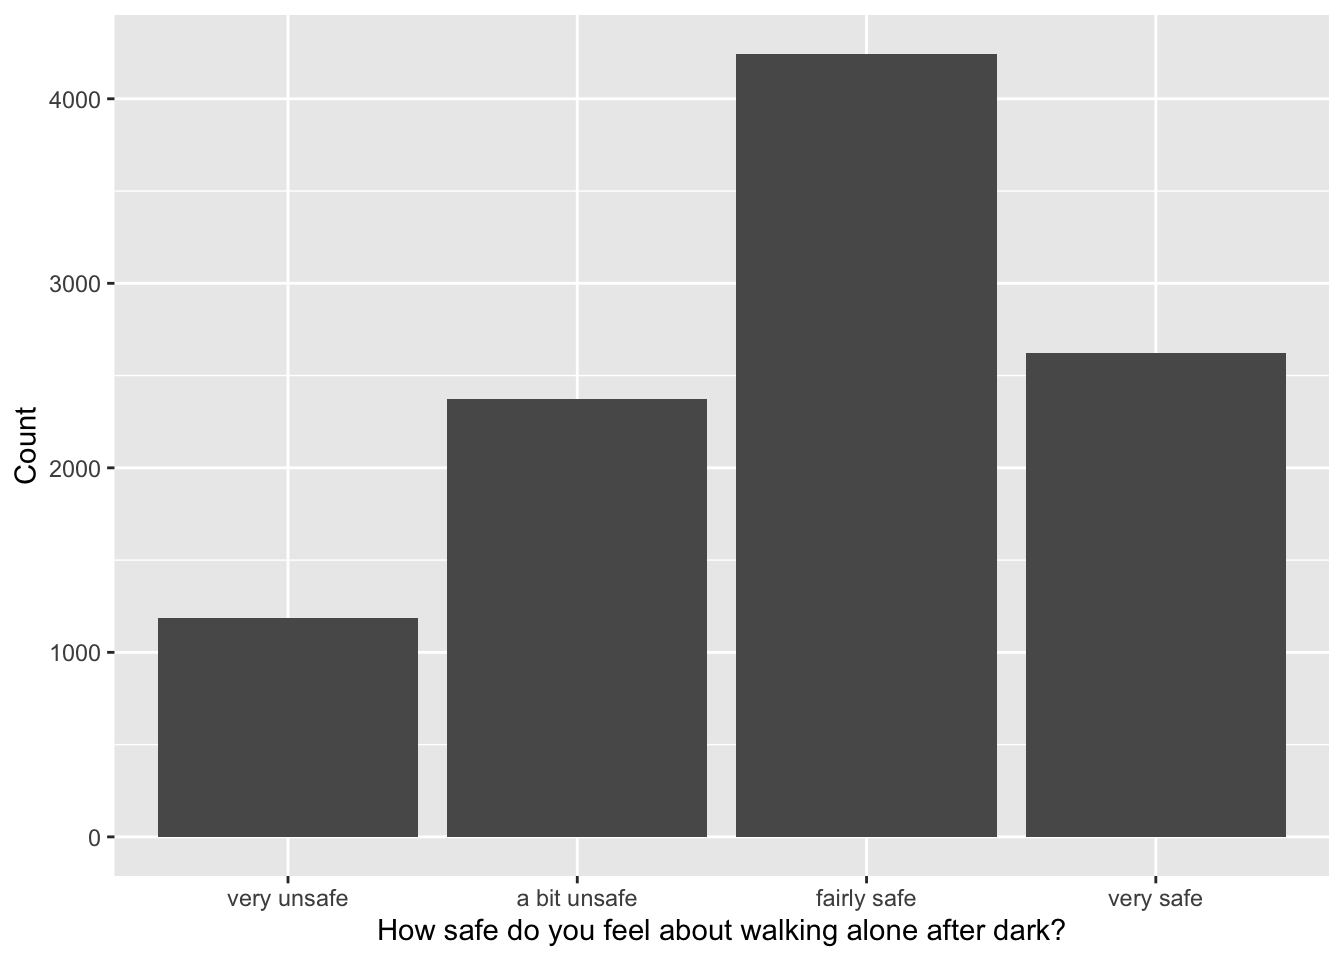
\includegraphics{_main_files/figure-latex/plot_walkdark-1.pdf}

A lot of people seem to feel at least fairly safe when walking alone after dark, but how does that response look like for different groups of people? Below is an example showing you how to separate the responses by sex:

\begin{Shaded}
\begin{Highlighting}[]
\FunctionTok{ggplot}\NormalTok{(}\AttributeTok{data=}\NormalTok{crimedata,}\FunctionTok{aes}\NormalTok{(walkdark,}\AttributeTok{fill=}\NormalTok{sex)) }\SpecialCharTok{+} \FunctionTok{geom\_bar}\NormalTok{(}\AttributeTok{position=}\StringTok{"dodge"}\NormalTok{) }\SpecialCharTok{+} \FunctionTok{xlab}\NormalTok{(}\StringTok{"How safe do you feel about walking alone after dark?"}\NormalTok{) }\SpecialCharTok{+} \FunctionTok{ylab}\NormalTok{(}\StringTok{"Count"}\NormalTok{)}
\end{Highlighting}
\end{Shaded}

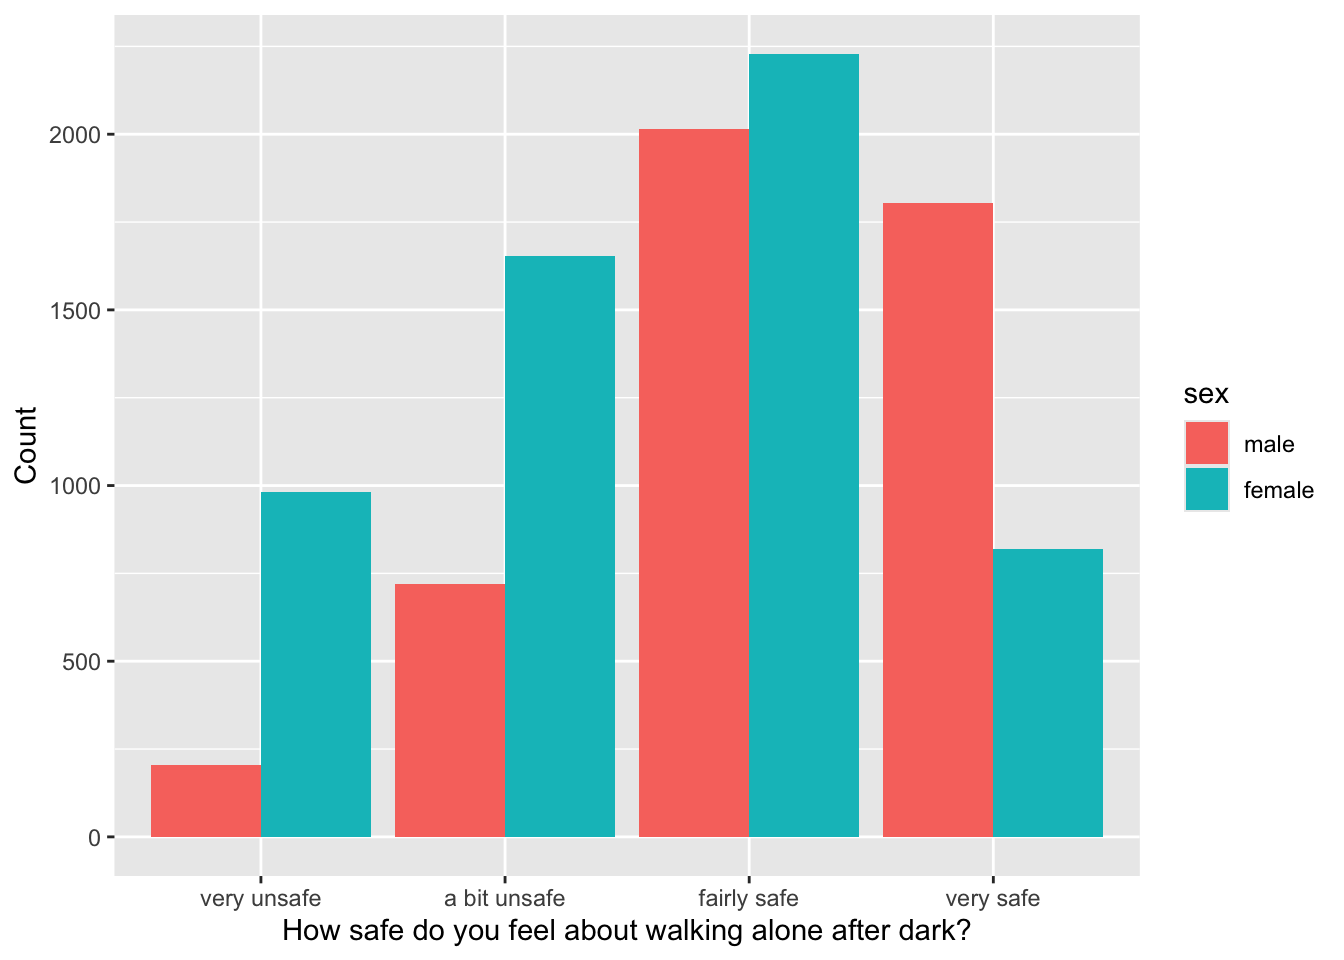
\includegraphics{_main_files/figure-latex/plot_walkdark_sex-1.pdf}

Note that in the code above, the function \texttt{geom\_bar()} creates a barplot and the argument \texttt{position="dodge"} specifies that the bars are supposed to appear side-by-side. Choosing \texttt{position="fill"} would give you a stacked barplot instead.

\textbf{How do you interpret the barplot of responses to walking alone after dark, by females and males?}

\begin{itemize}
\item
  \begin{enumerate}
  \def\labelenumi{(\Alph{enumi})}
  \tightlist
  \item
    Females tend to feel less safe than males walking alone after dark.\\
  \end{enumerate}
\item
  \begin{enumerate}
  \def\labelenumi{(\Alph{enumi})}
  \setcounter{enumi}{1}
  \tightlist
  \item
    Males tend to feel less safe than females walking alone after dark.\\
  \end{enumerate}
\item
  \begin{enumerate}
  \def\labelenumi{(\Alph{enumi})}
  \setcounter{enumi}{2}
  \tightlist
  \item
    The two sexes seem to feel similar about walking alone after dark.
  \end{enumerate}
\end{itemize}

Note that the plot shows the counts for each sex side-by-side. Since the number of female and male respondents might not be the same, it would be useful to know how many of each sex responded to the survey. You can find out via the function \texttt{table()}, as presented below:

\begin{Shaded}
\begin{Highlighting}[]
\FunctionTok{table}\NormalTok{(crimedata}\SpecialCharTok{$}\NormalTok{sex)}
\end{Highlighting}
\end{Shaded}

\begin{verbatim}
## 
##   male female 
##   4743   5684
\end{verbatim}

The survey contains quite a few more responses from females than males. Hence, the following plot might give a better insight to how the two sexes feel about walking alone after dark:

\begin{Shaded}
\begin{Highlighting}[]
\CommentTok{\#the argument position="fill" gives you a stacked barplot}
\FunctionTok{ggplot}\NormalTok{(}\AttributeTok{data=}\NormalTok{crimedata,}\FunctionTok{aes}\NormalTok{(sex,}\AttributeTok{fill=}\NormalTok{walkdark)) }\SpecialCharTok{+} \FunctionTok{geom\_bar}\NormalTok{(}\AttributeTok{position=}\StringTok{"fill"}\NormalTok{) }\SpecialCharTok{+} \FunctionTok{xlab}\NormalTok{(}\StringTok{"Sex"}\NormalTok{) }\SpecialCharTok{+} \FunctionTok{ylab}\NormalTok{(}\StringTok{"Proportion"}\NormalTok{) }\SpecialCharTok{+} \FunctionTok{ggtitle}\NormalTok{(}\StringTok{"How safe do you feel walking alone after dark?"}\NormalTok{) }\SpecialCharTok{+} \FunctionTok{labs}\NormalTok{(}\AttributeTok{fill=}\StringTok{\textquotesingle{}\textquotesingle{}}\NormalTok{)}
\end{Highlighting}
\end{Shaded}

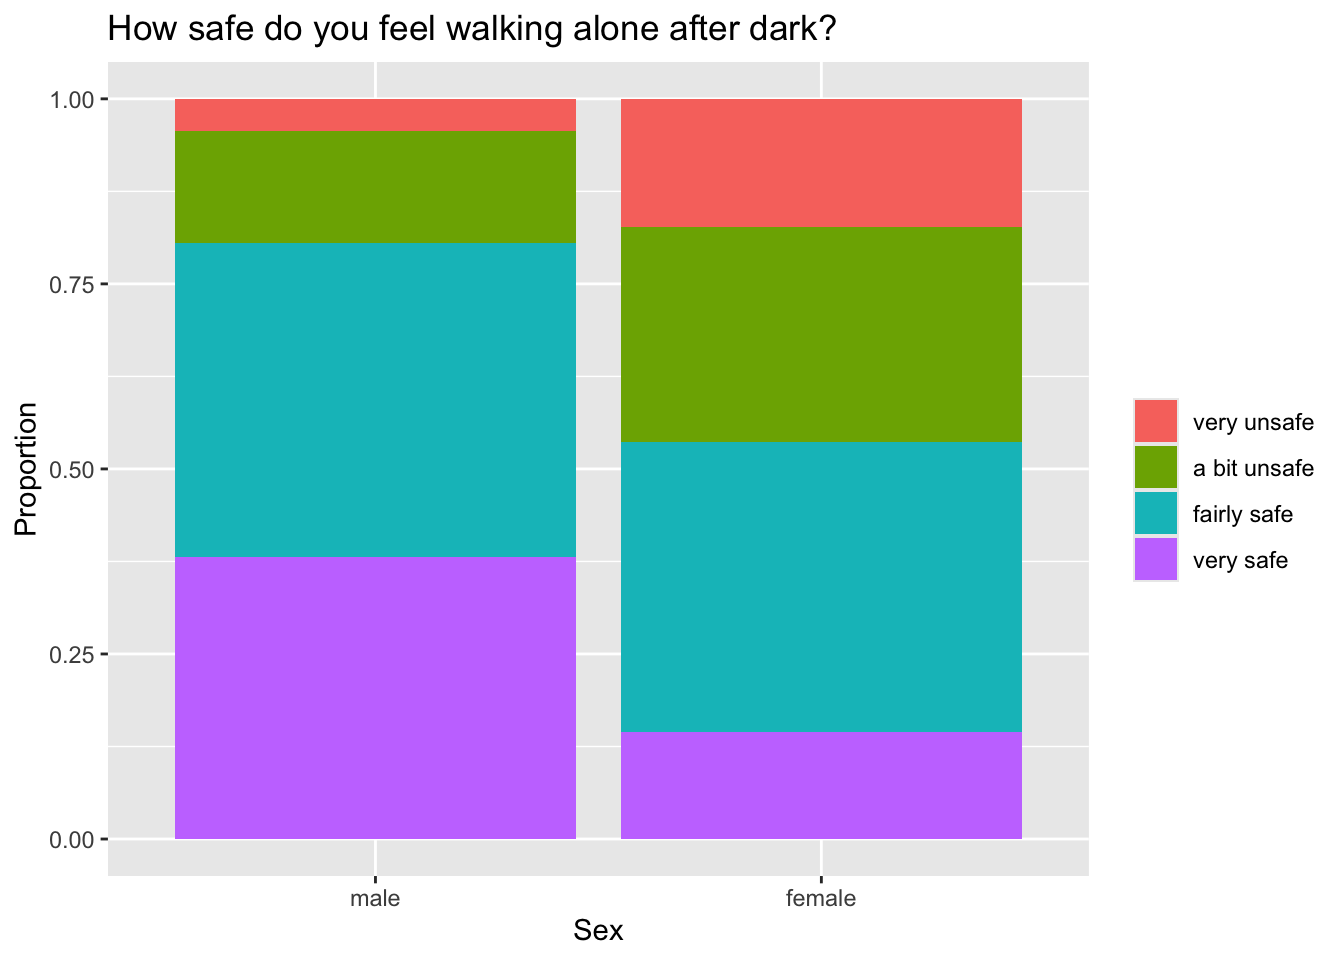
\includegraphics{_main_files/figure-latex/plot_walkdark_sex2-1.pdf}

Now, you can repeat the steps above for the variables \texttt{deprivation\_quintile}, \texttt{years\_in\_area}, \texttt{marital\_status} and \texttt{urban\_rural}, then answer the questions below.

\textbf{How would you describe a possible relationship between the deprivation quantiles and how safe people feel walking alone after dark?}

\begin{itemize}
\item
  \begin{enumerate}
  \def\labelenumi{(\Alph{enumi})}
  \tightlist
  \item
    It seems that the more deprived an area is, the more unsafe people feel about walking alone after dark.\\
  \end{enumerate}
\item
  \begin{enumerate}
  \def\labelenumi{(\Alph{enumi})}
  \setcounter{enumi}{1}
  \tightlist
  \item
    There is no apparent relationship between deprivation and how safe people feel walking alone after dark.\\
  \end{enumerate}
\item
  \begin{enumerate}
  \def\labelenumi{(\Alph{enumi})}
  \setcounter{enumi}{2}
  \tightlist
  \item
    It seems that the less deprived an area is, the more unsafe people feel about walking alone after dark.
  \end{enumerate}
\end{itemize}

Solution

\begin{Shaded}
\begin{Highlighting}[]
\FunctionTok{ggplot}\NormalTok{(}\AttributeTok{data=}\NormalTok{crimedata,}\FunctionTok{aes}\NormalTok{(deprivation\_quintile,}\AttributeTok{fill=}\NormalTok{walkdark)) }\SpecialCharTok{+} \FunctionTok{geom\_bar}\NormalTok{(}\AttributeTok{position=}\StringTok{"fill"}\NormalTok{) }\SpecialCharTok{+}
  \FunctionTok{xlab}\NormalTok{(}\StringTok{"Deprivation Quintile"}\NormalTok{) }\SpecialCharTok{+} \FunctionTok{ylab}\NormalTok{(}\StringTok{"Proportion"}\NormalTok{) }\SpecialCharTok{+}
  \FunctionTok{labs}\NormalTok{(}\AttributeTok{fill=}\StringTok{\textquotesingle{}\textquotesingle{}}\NormalTok{) }\SpecialCharTok{+} \FunctionTok{ggtitle}\NormalTok{(}\StringTok{"How safe do you feel walking alone after dark?"}\NormalTok{) }\SpecialCharTok{+} \FunctionTok{theme}\NormalTok{(}\AttributeTok{axis.text.x =} \FunctionTok{element\_text}\NormalTok{(}\AttributeTok{angle =} \DecValTok{90}\NormalTok{, }\AttributeTok{vjust =} \FloatTok{0.5}\NormalTok{, }\AttributeTok{hjust=}\DecValTok{1}\NormalTok{))}
\end{Highlighting}
\end{Shaded}

\textbf{How would you describe a possible relationship between the number of years people have lived in an area and how safe they feel walking alone after dark?}

\begin{itemize}
\item
  \begin{enumerate}
  \def\labelenumi{(\Alph{enumi})}
  \tightlist
  \item
    It seems that the longer a person has lived in an area, the less safe they feel about walking alone after dark.\\
  \end{enumerate}
\item
  \begin{enumerate}
  \def\labelenumi{(\Alph{enumi})}
  \setcounter{enumi}{1}
  \tightlist
  \item
    It seems that the longer a person has lived in an area, the more safe they feel about walking alone after dark.\\
  \end{enumerate}
\item
  \begin{enumerate}
  \def\labelenumi{(\Alph{enumi})}
  \setcounter{enumi}{2}
  \tightlist
  \item
    There is no apparent relationship between the number of years lived in an area and how safe people feel walking alone after dark.
  \end{enumerate}
\end{itemize}

Solution

\begin{Shaded}
\begin{Highlighting}[]
\FunctionTok{ggplot}\NormalTok{(}\AttributeTok{data=}\NormalTok{crimedata,}\FunctionTok{aes}\NormalTok{(years\_in\_area,}\AttributeTok{fill=}\NormalTok{walkdark)) }\SpecialCharTok{+} \FunctionTok{geom\_bar}\NormalTok{(}\AttributeTok{position=}\StringTok{"fill"}\NormalTok{) }\SpecialCharTok{+}
  \FunctionTok{xlab}\NormalTok{(}\StringTok{"Years in the area"}\NormalTok{) }\SpecialCharTok{+} \FunctionTok{ylab}\NormalTok{(}\StringTok{"Proportion"}\NormalTok{) }\SpecialCharTok{+}
  \FunctionTok{labs}\NormalTok{(}\AttributeTok{fill=}\StringTok{\textquotesingle{}\textquotesingle{}}\NormalTok{) }\SpecialCharTok{+} \FunctionTok{ggtitle}\NormalTok{(}\StringTok{"How safe do you feel walking alone after dark?"}\NormalTok{)}
\end{Highlighting}
\end{Shaded}

\textbf{What can you say about possible relationships between a person's marital status and how safe they feel walking alone after dark?}

\begin{itemize}
\item
  \begin{enumerate}
  \def\labelenumi{(\Alph{enumi})}
  \tightlist
  \item
    It seems that widowed people might feel more unsafe than the other groups.\\
  \end{enumerate}
\item
  \begin{enumerate}
  \def\labelenumi{(\Alph{enumi})}
  \setcounter{enumi}{1}
  \tightlist
  \item
    It seems that single people feel more safe than the other groups.\\
  \end{enumerate}
\item
  \begin{enumerate}
  \def\labelenumi{(\Alph{enumi})}
  \setcounter{enumi}{2}
  \tightlist
  \item
    It seems that married people feel more unsafe than single people.\\
  \end{enumerate}
\item
  \begin{enumerate}
  \def\labelenumi{(\Alph{enumi})}
  \setcounter{enumi}{3}
  \tightlist
  \item
    There are no apparent differences by marital status for how safe people feel walking alone after dark.
  \end{enumerate}
\end{itemize}

Solution

\begin{Shaded}
\begin{Highlighting}[]
\FunctionTok{ggplot}\NormalTok{(}\AttributeTok{data=}\NormalTok{crimedata,}\FunctionTok{aes}\NormalTok{(marital\_status,}\AttributeTok{fill=}\NormalTok{walkdark)) }\SpecialCharTok{+} \FunctionTok{geom\_bar}\NormalTok{(}\AttributeTok{position=}\StringTok{"fill"}\NormalTok{) }\SpecialCharTok{+}
  \FunctionTok{xlab}\NormalTok{(}\StringTok{"Marital Status"}\NormalTok{) }\SpecialCharTok{+} \FunctionTok{ylab}\NormalTok{(}\StringTok{"Proportion"}\NormalTok{) }\SpecialCharTok{+}
  \FunctionTok{labs}\NormalTok{(}\AttributeTok{fill=}\StringTok{\textquotesingle{}\textquotesingle{}}\NormalTok{) }\SpecialCharTok{+} \FunctionTok{ggtitle}\NormalTok{(}\StringTok{"How safe do you feel walking alone after dark?"}\NormalTok{)}
\end{Highlighting}
\end{Shaded}

\textbf{How do urban and rural areas compare for how safe people feel walking alone after dark?}

\begin{itemize}
\item
  \begin{enumerate}
  \def\labelenumi{(\Alph{enumi})}
  \tightlist
  \item
    It seems that people in rural areas feel more safe.\\
  \end{enumerate}
\item
  \begin{enumerate}
  \def\labelenumi{(\Alph{enumi})}
  \setcounter{enumi}{1}
  \tightlist
  \item
    It seems that people in urban areas feel more safe.\\
  \end{enumerate}
\item
  \begin{enumerate}
  \def\labelenumi{(\Alph{enumi})}
  \setcounter{enumi}{2}
  \tightlist
  \item
    People in urban and rural areas feel similarly safe walking alone after dark.
  \end{enumerate}
\end{itemize}

Solution

\begin{Shaded}
\begin{Highlighting}[]
\FunctionTok{ggplot}\NormalTok{(}\AttributeTok{data=}\NormalTok{crimedata,}\FunctionTok{aes}\NormalTok{(urban\_rural,}\AttributeTok{fill=}\NormalTok{walkdark)) }\SpecialCharTok{+} \FunctionTok{geom\_bar}\NormalTok{(}\AttributeTok{position=}\StringTok{"fill"}\NormalTok{) }\SpecialCharTok{+}
  \FunctionTok{xlab}\NormalTok{(}\StringTok{"Urban/Rural"}\NormalTok{) }\SpecialCharTok{+} \FunctionTok{ylab}\NormalTok{(}\StringTok{"Proportion"}\NormalTok{) }\SpecialCharTok{+}
  \FunctionTok{labs}\NormalTok{(}\AttributeTok{fill=}\StringTok{\textquotesingle{}\textquotesingle{}}\NormalTok{) }\SpecialCharTok{+} \FunctionTok{ggtitle}\NormalTok{(}\StringTok{"How safe do you feel walking alone after dark?"}\NormalTok{)}
\end{Highlighting}
\end{Shaded}

To compare responses by group, it might be helpful to obtain numerical summaries. For example, the code below shows you the number of males and females who live in urban and rural areas, respectively.

\begin{Shaded}
\begin{Highlighting}[]
\FunctionTok{table}\NormalTok{(crimedata}\SpecialCharTok{$}\NormalTok{sex,crimedata}\SpecialCharTok{$}\NormalTok{urban\_rural)}
\end{Highlighting}
\end{Shaded}

\begin{verbatim}
##         
##          urban rural
##   male    3604  1139
##   female  4342  1342
\end{verbatim}

You can compute frequencies from the table above using the following code:

\begin{Shaded}
\begin{Highlighting}[]
\NormalTok{sexurb }\OtherTok{\textless{}{-}} \FunctionTok{table}\NormalTok{(crimedata}\SpecialCharTok{$}\NormalTok{sex,crimedata}\SpecialCharTok{$}\NormalTok{urban\_rural)}
\CommentTok{\#proportion of males living in urban areas: }
\CommentTok{\#value from first row and column, divided by sum of first row}
\NormalTok{sexurb[}\DecValTok{1}\NormalTok{,}\DecValTok{1}\NormalTok{]}\SpecialCharTok{/}\FunctionTok{sum}\NormalTok{(sexurb[}\DecValTok{1}\NormalTok{,])}
\end{Highlighting}
\end{Shaded}

\begin{verbatim}
## [1] 0.7598566
\end{verbatim}

\begin{Shaded}
\begin{Highlighting}[]
\CommentTok{\#proportion of females living in urban areas:}
\NormalTok{sexurb[}\DecValTok{2}\NormalTok{,}\DecValTok{1}\NormalTok{]}\SpecialCharTok{/}\FunctionTok{sum}\NormalTok{(sexurb[}\DecValTok{2}\NormalTok{,])}
\end{Highlighting}
\end{Shaded}

\begin{verbatim}
## [1] 0.7638987
\end{verbatim}

Alternatively, you can first split the data into different groups and then compute the frequencies for the different datasets:

\begin{Shaded}
\begin{Highlighting}[]
\CommentTok{\#create a dataset for females only}
\NormalTok{fem }\OtherTok{\textless{}{-}}\NormalTok{ crimedata }\SpecialCharTok{\%\textgreater{}\%} \FunctionTok{filter}\NormalTok{(sex}\SpecialCharTok{==}\StringTok{"female"}\NormalTok{)}
\CommentTok{\#then divide the number of females living in urban areas by the number of females in total}
\FunctionTok{sum}\NormalTok{(fem}\SpecialCharTok{$}\NormalTok{urban\_rural}\SpecialCharTok{==}\StringTok{"urban"}\NormalTok{)}\SpecialCharTok{/}\FunctionTok{nrow}\NormalTok{(fem)}
\end{Highlighting}
\end{Shaded}

\begin{verbatim}
## [1] 0.7638987
\end{verbatim}

\textbf{You randomly select an individual from the crime data. What is the probability that the individual is married? (Round to 4 decimal places)}

Hint

Since you select the individual randomly, this probability can be computed as the number of married individuals divided by the total number of individuals.

\begin{center}\rule{0.5\linewidth}{0.5pt}\end{center}

Solution

\begin{Shaded}
\begin{Highlighting}[]
\CommentTok{\#solution}
\NormalTok{marital }\OtherTok{\textless{}{-}} \FunctionTok{table}\NormalTok{(crimedata}\SpecialCharTok{$}\NormalTok{marital\_status)}
\CommentTok{\#probability of randomly selected individual being married:}
\NormalTok{marital[}\DecValTok{1}\NormalTok{]}\SpecialCharTok{/}\FunctionTok{sum}\NormalTok{(marital)}
\end{Highlighting}
\end{Shaded}

\begin{verbatim}
##   married 
## 0.4753045
\end{verbatim}

\textbf{You randomly select a female from the crime data. What is the probability she is feeling very unsafe walking alone after dark?}

Hint

You randomly select an individual and you already know that the individual is female. Hence, the probability of her feeling very unsafe is the same as the proportion of females who feel very unsafe walking alone after dark.

\begin{center}\rule{0.5\linewidth}{0.5pt}\end{center}

Solution

\begin{Shaded}
\begin{Highlighting}[]
\CommentTok{\#solution}
\NormalTok{femdark }\OtherTok{\textless{}{-}} \FunctionTok{table}\NormalTok{(crimedata}\SpecialCharTok{$}\NormalTok{sex,crimedata}\SpecialCharTok{$}\NormalTok{walkdark)}
\CommentTok{\#probability of randomly selected female feeling very unsafe:}
\NormalTok{femdark[}\DecValTok{2}\NormalTok{,}\DecValTok{1}\NormalTok{]}\SpecialCharTok{/}\FunctionTok{sum}\NormalTok{(femdark[}\DecValTok{2}\NormalTok{,])}
\end{Highlighting}
\end{Shaded}

\begin{verbatim}
## [1] 0.1727657
\end{verbatim}

\textbf{Compute the proportions of widowed females and widowed males who feel very unsafe walking alone after dark. Without performing a formal hypothesis test, would you suggest that these proportions differ substantially?}

\begin{itemize}
\item
  \begin{enumerate}
  \def\labelenumi{(\Alph{enumi})}
  \tightlist
  \item
    Yes, the proportion of people who feel very unsafe walking alone after dark appears to be higher in widowed females than widowed males.\\
  \end{enumerate}
\item
  \begin{enumerate}
  \def\labelenumi{(\Alph{enumi})}
  \setcounter{enumi}{1}
  \tightlist
  \item
    Yes, the proportion of people who feel very unsafe walking alone after dark appears to be higher in widowed males than widowed females.\\
  \end{enumerate}
\item
  \begin{enumerate}
  \def\labelenumi{(\Alph{enumi})}
  \setcounter{enumi}{2}
  \tightlist
  \item
    No, the proportions are about the same.
  \end{enumerate}
\end{itemize}

Solution

\begin{Shaded}
\begin{Highlighting}[]
\CommentTok{\#solution to the multiple choice question above}
\NormalTok{femwidowed }\OtherTok{\textless{}{-}}\NormalTok{ crimedata }\SpecialCharTok{\%\textgreater{}\%} \FunctionTok{filter}\NormalTok{(sex}\SpecialCharTok{==}\StringTok{"female"} \SpecialCharTok{\&}\NormalTok{ marital\_status}\SpecialCharTok{==}\StringTok{"widowed"}\NormalTok{)}
\CommentTok{\#proportions of widowed females feeling very unsafe walking alone after dark}
\FunctionTok{sum}\NormalTok{(femwidowed}\SpecialCharTok{$}\NormalTok{walkdark}\SpecialCharTok{==}\StringTok{"very unsafe"}\NormalTok{)}\SpecialCharTok{/}\FunctionTok{nrow}\NormalTok{(femwidowed)}
\end{Highlighting}
\end{Shaded}

\begin{verbatim}
## [1] 0.3033839
\end{verbatim}

\begin{Shaded}
\begin{Highlighting}[]
\NormalTok{malwidowed }\OtherTok{\textless{}{-}}\NormalTok{ crimedata }\SpecialCharTok{\%\textgreater{}\%} \FunctionTok{filter}\NormalTok{(sex}\SpecialCharTok{==}\StringTok{"male"} \SpecialCharTok{\&}\NormalTok{ marital\_status}\SpecialCharTok{==}\StringTok{"widowed"}\NormalTok{)}
\CommentTok{\#proportions of widowed females feeling very unsafe walking alone after dark}
\FunctionTok{sum}\NormalTok{(malwidowed}\SpecialCharTok{$}\NormalTok{walkdark}\SpecialCharTok{==}\StringTok{"very unsafe"}\NormalTok{)}\SpecialCharTok{/}\FunctionTok{nrow}\NormalTok{(malwidowed)}
\end{Highlighting}
\end{Shaded}

\begin{verbatim}
## [1] 0.09459459
\end{verbatim}

Hopefully, this part of the lab gave you some good ideas how to use plots to gain insights for a given dataset. If you want, you can explore the crime data further by checking possible associations between other variables in the data.

\hypertarget{part-2---probability}{%
\chapter{Part 2 - Probability}\label{part-2---probability}}

\hypertarget{the-normal-distribution}{%
\subsection{The normal distribution}\label{the-normal-distribution}}

In the lecture, you were introduced to the normal distribution and how to use the Z-table to look up cumulative proabilities or percentiles of the standard normal distribution \(N(\mu=0,\sigma=1)\). These tables were particularly useful before computers were invented or whenever they are unavailable to you (for example, when you are stranded on an island\ldots{} or when you are sitting a closed-book exam).

In \texttt{R}, you can compute cumulative probabilities and percentiles directly from the normal distribution, rather than having to approximate them using the tables. You can get an overview of the different functions available by calling the help function:

\begin{Shaded}
\begin{Highlighting}[]
\NormalTok{?Normal}
\end{Highlighting}
\end{Shaded}

If you want to compute the cumulative probability of a variable \(X\)\textasciitilde{}\(N(\mu=3,\sigma=2)\), e.g.~\(P(X \leq 2)\), this can be done using the following line of code:

\begin{Shaded}
\begin{Highlighting}[]
\FunctionTok{pnorm}\NormalTok{(}\AttributeTok{q=}\DecValTok{2}\NormalTok{,}\AttributeTok{mean=}\DecValTok{3}\NormalTok{,}\AttributeTok{sd=}\DecValTok{2}\NormalTok{)}
\end{Highlighting}
\end{Shaded}

\begin{verbatim}
## [1] 0.3085375
\end{verbatim}

To confirm this result, you can compute the Z-score \(\left(Z=\frac{X-\mu}{\sigma}\right)\) of \(X=2\) and look up the cumulative probability in the Z-table.

If you want to find the 95th percentile of the variable \(X\)\textasciitilde{}\(N(\mu=3,\sigma=2)\), you can do so by typing the following:

\begin{Shaded}
\begin{Highlighting}[]
\FunctionTok{qnorm}\NormalTok{(}\AttributeTok{p=}\FloatTok{0.95}\NormalTok{,}\AttributeTok{mean=}\DecValTok{3}\NormalTok{,}\AttributeTok{sd=}\DecValTok{2}\NormalTok{)}
\end{Highlighting}
\end{Shaded}

\begin{verbatim}
## [1] 6.289707
\end{verbatim}

Again, you can confirm the result by looking up the Z-score belonging to the 95th percentile of the standard normal distribution and back-transform to obtain the corresponding value of \(X\).

\textbf{For \(X\)\textasciitilde{}\(N(\mu=82,\sigma=7)\), what is \(P(X<90)\)? (Round to 4 decimal places)}

Hint

pnorm(q=?,mean=?,sd=?)

\begin{center}\rule{0.5\linewidth}{0.5pt}\end{center}

Solution

\begin{Shaded}
\begin{Highlighting}[]
\CommentTok{\#P(X\textless{}90)=P(X≤90) for continuous variables}
\FunctionTok{pnorm}\NormalTok{(}\AttributeTok{q=}\DecValTok{90}\NormalTok{,}\AttributeTok{mean=}\DecValTok{82}\NormalTok{,}\AttributeTok{sd=}\DecValTok{7}\NormalTok{)}
\end{Highlighting}
\end{Shaded}

\begin{verbatim}
## [1] 0.873451
\end{verbatim}

\textbf{For \(X\)\textasciitilde{}\(N(\mu=82,\sigma=7)\), what is \(P(X>73)\)? (Round to 4 decimal places)}

Hint 1

What is the complement of \(X>73\)?

Hint 2

Apply pnorm() to the complementary event, i.e.~compute
1-pnorm(q=?,mean=?,sd=?)

\begin{center}\rule{0.5\linewidth}{0.5pt}\end{center}

Solution

\begin{Shaded}
\begin{Highlighting}[]
\CommentTok{\#P(X\textgreater{}73)=1{-}P(X\textless{}73)=1{-}P(X≤73)}
\DecValTok{1}\SpecialCharTok{{-}}\FunctionTok{pnorm}\NormalTok{(}\AttributeTok{q=}\DecValTok{73}\NormalTok{,}\AttributeTok{mean=}\DecValTok{82}\NormalTok{,}\AttributeTok{sd=}\DecValTok{7}\NormalTok{)}
\end{Highlighting}
\end{Shaded}

\begin{verbatim}
## [1] 0.9007286
\end{verbatim}

\begin{Shaded}
\begin{Highlighting}[]
\CommentTok{\#or alternatively, you can specify lower.tail=FALSE to compute P(X\textgreater{}73) directly:}
\FunctionTok{pnorm}\NormalTok{(}\AttributeTok{q=}\DecValTok{73}\NormalTok{,}\AttributeTok{mean=}\DecValTok{82}\NormalTok{,}\AttributeTok{sd=}\DecValTok{7}\NormalTok{,}\AttributeTok{lower.tail=}\ConstantTok{FALSE}\NormalTok{)}
\end{Highlighting}
\end{Shaded}

\begin{verbatim}
## [1] 0.9007286
\end{verbatim}

\textbf{For \(X\)\textasciitilde{}\(N(\mu=82,\sigma=7)\), what is \(P(73<X<90)\)? (Round to 4 decimal places)}

Hint

pnorm(q=?,mean=?,sd=?) - pnorm(q=?,mean=?,sd=?)

\begin{center}\rule{0.5\linewidth}{0.5pt}\end{center}

Solution

\begin{Shaded}
\begin{Highlighting}[]
\CommentTok{\#P(73\textless{}X\textless{}90)}
\FunctionTok{pnorm}\NormalTok{(}\AttributeTok{q=}\DecValTok{90}\NormalTok{,}\AttributeTok{mean=}\DecValTok{82}\NormalTok{,}\AttributeTok{sd=}\DecValTok{7}\NormalTok{)}\SpecialCharTok{{-}}\FunctionTok{pnorm}\NormalTok{(}\AttributeTok{q=}\DecValTok{73}\NormalTok{,}\AttributeTok{mean=}\DecValTok{82}\NormalTok{,}\AttributeTok{sd=}\DecValTok{7}\NormalTok{)}
\end{Highlighting}
\end{Shaded}

\begin{verbatim}
## [1] 0.7741796
\end{verbatim}

\textbf{For \(X\)\textasciitilde{}\(N(\mu=12,\sigma=3)\), what is the 95th percentile? (Round to 2 decimal places)}

Hint

qnorm(p=?,mean=?,sd=?)

\begin{center}\rule{0.5\linewidth}{0.5pt}\end{center}

Solution

\begin{Shaded}
\begin{Highlighting}[]
\CommentTok{\#95th percentile}
\FunctionTok{qnorm}\NormalTok{(}\AttributeTok{p=}\FloatTok{0.95}\NormalTok{,}\AttributeTok{mean=}\DecValTok{12}\NormalTok{,}\AttributeTok{sd=}\DecValTok{3}\NormalTok{)}
\end{Highlighting}
\end{Shaded}

\begin{verbatim}
## [1] 16.93456
\end{verbatim}

\textbf{For \(X\)\textasciitilde{}\(N(\mu=12,\sigma=3)\), what is the 10th percentile? (Round to 2 decimal places)}

Hint

qnorm(p=?,mean=?,sd=?)

\begin{center}\rule{0.5\linewidth}{0.5pt}\end{center}

Solution

\begin{Shaded}
\begin{Highlighting}[]
\CommentTok{\#10th percentile}
\FunctionTok{qnorm}\NormalTok{(}\AttributeTok{p=}\FloatTok{0.1}\NormalTok{,}\AttributeTok{mean=}\DecValTok{12}\NormalTok{,}\AttributeTok{sd=}\DecValTok{3}\NormalTok{)}
\end{Highlighting}
\end{Shaded}

\begin{verbatim}
## [1] 8.155345
\end{verbatim}

\hypertarget{discrete-distributions}{%
\subsection{Discrete distributions}\label{discrete-distributions}}

Similar to the normal distribution, you can use \texttt{R} to compute cumulative probabilities and percentiles for the binomial and Poisson distributions. Additionally, you can evaluate the probability mass functions of these distributions for particular values that the random variables might take on. The probability mass functions are evaluated with the functions \texttt{dbinom()} and \texttt{dpois()}. The cumulative probabilities are computed with \texttt{pbinom()} and \texttt{ppois()}, and the percentiles are computed with \texttt{qbinom()} and \texttt{qpois()}. You can call the help functions below to get additional info on how to use these functions:

\begin{Shaded}
\begin{Highlighting}[]
\NormalTok{?Binomial}
\NormalTok{?Poisson}
\end{Highlighting}
\end{Shaded}

Note that functions for the geometric and negative binomial distributions exist in the standard \texttt{R} package. However, in \texttt{R}, these distributions are defined slightly differently from how we covered them in the lecture. Hence, I recommend you \textbf{do not} use the built-in function and instead use the lines of code provided in the exercises below.

\hypertarget{binomial}{%
\subsubsection{Binomial}\label{binomial}}

\textbf{For \(X \sim \mbox{Bin}(n=30,\theta=0.1)\), what is \(P(X=4)\)? (Round to 4 decimal places)}

Hint

dbinom(x=?,size=?,prob=?)

\begin{center}\rule{0.5\linewidth}{0.5pt}\end{center}

Solution

\begin{Shaded}
\begin{Highlighting}[]
\CommentTok{\#P(X=4)}
\FunctionTok{dbinom}\NormalTok{(}\AttributeTok{x=}\DecValTok{4}\NormalTok{,}\AttributeTok{size=}\DecValTok{30}\NormalTok{,}\AttributeTok{prob=}\FloatTok{0.1}\NormalTok{)}
\end{Highlighting}
\end{Shaded}

\begin{verbatim}
## [1] 0.1770659
\end{verbatim}

\textbf{For \(X \sim \mbox{Bin}(n=10,\theta=0.3)\), what is \(P(X<5)\)? (Round to 4 decimal places)}

Hint

pbinom(x=?,size=?,prob=?)

\begin{center}\rule{0.5\linewidth}{0.5pt}\end{center}

Solution

\begin{Shaded}
\begin{Highlighting}[]
\CommentTok{\#P(X\textless{}5)=P(X≤4) for discrete variables}
\FunctionTok{pbinom}\NormalTok{(}\AttributeTok{q=}\DecValTok{4}\NormalTok{,}\AttributeTok{size=}\DecValTok{10}\NormalTok{,}\AttributeTok{prob=}\FloatTok{0.3}\NormalTok{)}
\end{Highlighting}
\end{Shaded}

\begin{verbatim}
## [1] 0.8497317
\end{verbatim}

\textbf{For \(X \sim \mbox{Bin}(n=10,\theta=0.3)\), what is \(P(X>1)\)? (Round to 4 decimal places)}

Hint 1

What is the complementary event of \(X>1\)?

Hint 2

Apply pbinom() to the complementary event, i.e.~compute
1-pbinom(q=?,size=?,prob=?)

\begin{center}\rule{0.5\linewidth}{0.5pt}\end{center}

Solution

\begin{Shaded}
\begin{Highlighting}[]
\CommentTok{\#P(X\textgreater{}1)=1{-}P(X≤1)}
\DecValTok{1}\SpecialCharTok{{-}}\FunctionTok{pbinom}\NormalTok{(}\AttributeTok{q=}\DecValTok{1}\NormalTok{,}\AttributeTok{size=}\DecValTok{10}\NormalTok{,}\AttributeTok{prob=}\FloatTok{0.3}\NormalTok{)}
\end{Highlighting}
\end{Shaded}

\begin{verbatim}
## [1] 0.8506917
\end{verbatim}

\textbf{For \(X \sim \mbox{Bin}(n=10,\theta=0.3)\), what is \(P(1<X<5)\)? (Round to 4 decimal places)}

Hint

pbinom(q=?,size=?,prob=?)-pbinom(q=?,size=?,prob=?)

\begin{center}\rule{0.5\linewidth}{0.5pt}\end{center}

Solution

\begin{Shaded}
\begin{Highlighting}[]
\CommentTok{\#P(1\textless{}X\textless{}5)}
\FunctionTok{pbinom}\NormalTok{(}\AttributeTok{q=}\DecValTok{4}\NormalTok{,}\AttributeTok{size=}\DecValTok{10}\NormalTok{,}\AttributeTok{prob=}\FloatTok{0.3}\NormalTok{)}\SpecialCharTok{{-}}\FunctionTok{pbinom}\NormalTok{(}\AttributeTok{q=}\DecValTok{1}\NormalTok{,}\AttributeTok{size=}\DecValTok{10}\NormalTok{,}\AttributeTok{prob=}\FloatTok{0.3}\NormalTok{)}
\end{Highlighting}
\end{Shaded}

\begin{verbatim}
## [1] 0.7004233
\end{verbatim}

\textbf{For \(X \sim \mbox{Bin}(n=40,\theta=0.2)\), what is the 90th percentile? (As a whole number)}

Hint

qbinom(p=?,size=?,prob=?)

\_\_

Solution

\begin{Shaded}
\begin{Highlighting}[]
\FunctionTok{qbinom}\NormalTok{(}\AttributeTok{p=}\FloatTok{0.9}\NormalTok{,}\AttributeTok{size=}\DecValTok{40}\NormalTok{,}\AttributeTok{prob=}\FloatTok{0.2}\NormalTok{)}
\end{Highlighting}
\end{Shaded}

\begin{verbatim}
## [1] 11
\end{verbatim}

\hypertarget{geometric}{%
\subsubsection{Geometric}\label{geometric}}

The geometric distribution is defined differently in \texttt{R} than in our course. Hence, I recommend you compute probabilities from the geometric distribution using the formulas in the notes rather than the built-in functions. Luckily, the PMF and CDF of the geometric distribution are quickly computed without any built-in functions.

\textbf{For \(X \sim \mbox{Geom}(\theta=0.2)\), what is \(P(X=3)\)? (Round to 3 decimal places)}

Hint

Recall the PMF of a geometric random variable \(X\): \(P(X=x)=(1-\theta)^{(x-1)}\times \theta\)

\begin{center}\rule{0.5\linewidth}{0.5pt}\end{center}

Solution

\begin{Shaded}
\begin{Highlighting}[]
\FloatTok{0.8}\SpecialCharTok{\^{}}\DecValTok{2}\SpecialCharTok{*}\FloatTok{0.2}
\end{Highlighting}
\end{Shaded}

\begin{verbatim}
## [1] 0.128
\end{verbatim}

\textbf{For \(X \sim \mbox{Geom}(\theta=0.02)\), what is \(P(X>4)\)? (Round to 4 decimal places)}

Hint

Recall that for a geometric random variable \(X\), you can compute \(P(X>x)=(1-\theta)^{x}\).

\begin{center}\rule{0.5\linewidth}{0.5pt}\end{center}

Solution

\begin{Shaded}
\begin{Highlighting}[]
\NormalTok{(}\DecValTok{1}\FloatTok{{-}0.02}\NormalTok{)}\SpecialCharTok{\^{}}\DecValTok{4}
\end{Highlighting}
\end{Shaded}

\begin{verbatim}
## [1] 0.9223682
\end{verbatim}

\textbf{For \(X \sim \mbox{Geom}(\theta=0.02)\), what is \(P(X<20)\)? (Round to 4 decimal places)}

Hint

For a geometric random variable \(X\), it is easier to compute the probability of \(X\) being greater than some value \(x\): \(P(X>x)=(1-\theta)^{x}\). Now, you can compute \(P(X<20)=1-P(X>19)\).

\begin{center}\rule{0.5\linewidth}{0.5pt}\end{center}

Solution

\begin{Shaded}
\begin{Highlighting}[]
\DecValTok{1}\SpecialCharTok{{-}}\NormalTok{(}\DecValTok{1}\FloatTok{{-}0.02}\NormalTok{)}\SpecialCharTok{\^{}}\DecValTok{19}
\end{Highlighting}
\end{Shaded}

\begin{verbatim}
## [1] 0.3187674
\end{verbatim}

\textbf{For \(X \sim \mbox{Geom}(\theta=0.02)\), what is \(P(4<X<20)\)? (Round to 4 decimal places)}

Hint

\(P(4<X<20)=P(X<20)-P(X \leq 4)=(1-P(X>19))-(1-P(X>4))\)

\begin{center}\rule{0.5\linewidth}{0.5pt}\end{center}

Solution

\begin{Shaded}
\begin{Highlighting}[]
\NormalTok{(}\DecValTok{1}\SpecialCharTok{{-}}\NormalTok{(}\DecValTok{1}\FloatTok{{-}0.02}\NormalTok{)}\SpecialCharTok{\^{}}\DecValTok{19}\NormalTok{)}\SpecialCharTok{{-}}\NormalTok{(}\DecValTok{1}\SpecialCharTok{{-}}\NormalTok{(}\DecValTok{1}\FloatTok{{-}0.02}\NormalTok{)}\SpecialCharTok{\^{}}\DecValTok{4}\NormalTok{)}
\end{Highlighting}
\end{Shaded}

\begin{verbatim}
## [1] 0.2411355
\end{verbatim}

\hypertarget{negative-binomial}{%
\subsubsection{Negative binomial}\label{negative-binomial}}

Recall that for a negative binomial random variable \(X \sim \mbox{Neg.Bin.}(\theta)\), the PMF can be written as \begin{align*}
  P(X=x)&=\binom{x-1}{k-1}(1-\theta)^{(x-k)}\theta^{k}\\
  &=\binom{x-1}{k-1}(1-\theta)^{(x-k)}\theta^{k-1} \times \theta\\
  &=P(X_{1}=(k-1)) \times P(X_{2}=1),
\end{align*}

where \(X_{1} \sim \mbox{Bin}(n=(x-1),\theta)\) and \(X_{2} \sim \mbox{Bern}(\theta)\). You can use that trick to compute probabilities from the negative binomial distribution in \texttt{R}.

\textbf{For \(X \sim \mbox{Neg.Bin.}(\theta=0.1)\) and \(k=4\), what is \(P(X=10)\)? (Round to 4 decimal places)}

Hint

\(P(X=10)=P(X_{1}=3) \times P(X_{2}=1)\), for \(X_{1}\sim \mbox{Bin}(n=(x-1),\theta)\) and \(X_{2}\sim \mbox{Bern}(\theta)\).

Alternatively, you can use the formula for the negative binomial PMF.

\begin{center}\rule{0.5\linewidth}{0.5pt}\end{center}

Solution

\begin{Shaded}
\begin{Highlighting}[]
\CommentTok{\#using the hint:}
\FunctionTok{dbinom}\NormalTok{(}\AttributeTok{x=}\DecValTok{3}\NormalTok{,}\AttributeTok{size=}\DecValTok{9}\NormalTok{,}\AttributeTok{prob=}\FloatTok{0.1}\NormalTok{)}\SpecialCharTok{*}\FloatTok{0.1}
\end{Highlighting}
\end{Shaded}

\begin{verbatim}
## [1] 0.004464104
\end{verbatim}

\begin{Shaded}
\begin{Highlighting}[]
\CommentTok{\#or:}
\FunctionTok{choose}\NormalTok{(}\DecValTok{9}\NormalTok{,}\DecValTok{3}\NormalTok{)}\SpecialCharTok{*}\NormalTok{(}\DecValTok{1}\FloatTok{{-}0.1}\NormalTok{)}\SpecialCharTok{\^{}}\DecValTok{6}\SpecialCharTok{*}\FloatTok{0.1}\SpecialCharTok{\^{}}\DecValTok{4}
\end{Highlighting}
\end{Shaded}

\begin{verbatim}
## [1] 0.004464104
\end{verbatim}

\hypertarget{poisson}{%
\subsubsection{Poisson}\label{poisson}}

\textbf{For \(X \sim \mbox{Pois}(\lambda=3)\), what is what is \(P(X=2)\)? (Round to 3 decimal places)}

Hint

dpois(x=?,lambda=?)

\begin{center}\rule{0.5\linewidth}{0.5pt}\end{center}

Solution

\begin{Shaded}
\begin{Highlighting}[]
\FunctionTok{dpois}\NormalTok{(}\AttributeTok{x=}\DecValTok{2}\NormalTok{,}\AttributeTok{lambda=}\DecValTok{3}\NormalTok{)}
\end{Highlighting}
\end{Shaded}

\begin{verbatim}
## [1] 0.2240418
\end{verbatim}

\textbf{For \(X\sim \mbox{Pois}(\lambda=10)\), what is what is \(P(X<12)\)? (Round to 4 decimal places)}

Hint

ppois(q=?,lambda=?)

\begin{center}\rule{0.5\linewidth}{0.5pt}\end{center}

Solution

\begin{Shaded}
\begin{Highlighting}[]
\CommentTok{\#P(X\textless{}12)=P(X≤11) for discrete variables}
\FunctionTok{ppois}\NormalTok{(}\AttributeTok{q=}\DecValTok{11}\NormalTok{,}\AttributeTok{lambda=}\DecValTok{10}\NormalTok{)}
\end{Highlighting}
\end{Shaded}

\begin{verbatim}
## [1] 0.6967761
\end{verbatim}

\textbf{For \(X\sim \mbox{Pois}(\lambda=10)\), what is what is \(P(X>7)\)? (Round to 4 decimal places)}

Hint

What is the complement of \(X>7\)?

\begin{center}\rule{0.5\linewidth}{0.5pt}\end{center}

Solution

\begin{Shaded}
\begin{Highlighting}[]
\CommentTok{\#P(X\textgreater{}7)=1{-}P(X≤7)}
\DecValTok{1}\SpecialCharTok{{-}}\FunctionTok{ppois}\NormalTok{(}\AttributeTok{q=}\DecValTok{7}\NormalTok{,}\AttributeTok{lambda=}\DecValTok{10}\NormalTok{)}
\end{Highlighting}
\end{Shaded}

\begin{verbatim}
## [1] 0.7797794
\end{verbatim}

\textbf{For \(X\sim \mbox{Pois}(\lambda=10)\), what is what is \(P(7<X<12)\)? (Round to 4 decimal places)}

Hint

ppois(q=?,lambda=?) - ppois(q=?,lambda=?)

\begin{center}\rule{0.5\linewidth}{0.5pt}\end{center}

Solution

\begin{Shaded}
\begin{Highlighting}[]
\CommentTok{\#P(7\textless{}X\textless{}12)}
\FunctionTok{ppois}\NormalTok{(}\AttributeTok{q=}\DecValTok{11}\NormalTok{,}\AttributeTok{lambda=}\DecValTok{10}\NormalTok{)}\SpecialCharTok{{-}}\FunctionTok{ppois}\NormalTok{(}\AttributeTok{q=}\DecValTok{7}\NormalTok{,}\AttributeTok{lambda=}\DecValTok{10}\NormalTok{)}
\end{Highlighting}
\end{Shaded}

\begin{verbatim}
## [1] 0.4765555
\end{verbatim}

\textbf{For \(X\sim \mbox{Pois}(\lambda=7)\), what is what is the 95th percentile? (As a whole number)}

Hint

qpois(p=?,lambda=?)

\_\_

Solution

\begin{Shaded}
\begin{Highlighting}[]
\FunctionTok{qpois}\NormalTok{(}\AttributeTok{p=}\FloatTok{0.95}\NormalTok{,}\AttributeTok{lambda=}\DecValTok{7}\NormalTok{)}
\end{Highlighting}
\end{Shaded}

\begin{verbatim}
## [1] 12
\end{verbatim}

\hypertarget{using-the-normal-distribution-to-approximate-a-binomial-distribution}{%
\subsection{Using the normal distribution to approximate a binomial distribution}\label{using-the-normal-distribution-to-approximate-a-binomial-distribution}}

In lecture 16, you saw that the binomial distribution can be approximated by a normal distribution. Specifically, if \(n \times \theta \geq 10\) and \(n \times (1-\theta) \geq 10\), then \(X \sim \mbox{Bin}(n,\theta)\) can be approximated by
\begin{align*}
Y \sim N\left(\mu=n \times \theta,\sigma=\sqrt{n \times \theta \times (1-\theta)}\right)
\end{align*}

\textbf{For a binomial distribution with sample size 30 and probability of success equal to 0.2, would you suggest approximating the distribution by a normal distribution?}

Hint

Check if the assumptions \(n \times \theta \geq 10\) and \(n \times (1-\theta) \geq 10\) hold.

\begin{itemize}
\item
  \begin{enumerate}
  \def\labelenumi{(\Alph{enumi})}
  \tightlist
  \item
    Sure, why not?!\\
  \end{enumerate}
\item
  \begin{enumerate}
  \def\labelenumi{(\Alph{enumi})}
  \setcounter{enumi}{1}
  \tightlist
  \item
    No, because we can\textquotesingle t assume the binomial and normal distributions to be independent.\\
  \end{enumerate}
\item
  \begin{enumerate}
  \def\labelenumi{(\Alph{enumi})}
  \setcounter{enumi}{2}
  \tightlist
  \item
    No, the expected number of successes is too small, so the normal approximation should not be used.
  \end{enumerate}
\end{itemize}

\textbf{For \(X \sim \mbox{Bin}(n=400,\theta=0.1)\), fill in the blanks for the Normal approximation you would use:}

Hint

Recall that \(X\)\textasciitilde Binomial(\(n,\theta\)) can be approximated by \(Y\)\textasciitilde{}\(N\left(\mu=n \times \theta,\sigma=\sqrt{n \times \theta \times (1-\theta)}\right)\).

\(N(\mu=\)\_\_\(,\sigma=\)\_\()\).

Solution

\(\mu=n \times \theta=40\), \(\sigma=\sqrt{n \times \theta \times (1-\theta)}=\sqrt{36}=6\)

\hypertarget{graphical-exploration}{%
\subsubsection{Graphical exploration}\label{graphical-exploration}}

For the random variable \(X \sim \mbox{Bin}(n=600,\theta=0.4)\), you get \(n \times \theta=240>10\) and \(n \times (1-\theta)=360>10\), so it is appropriate to approximate the distribution using a normal distribution with mean \(\mu=n \times \theta=240\) and standard deviation \(\sigma=\sqrt{n \times \theta \times (1-\theta)}=\sqrt{144}=12\). To get a visual idea for how well the normal distribution approximates the binomial, you can create a plot that overlays the cumulative densities of the two distributions. You will need a sequence of numbers at which to evaluate the respective cumulative density functions (CDFs). This can be done using the \texttt{seq()} function, as demonstrated below:

\begin{Shaded}
\begin{Highlighting}[]
\FunctionTok{seq}\NormalTok{(}\AttributeTok{from=}\DecValTok{0}\NormalTok{,}\AttributeTok{to=}\DecValTok{10}\NormalTok{,}\AttributeTok{by=}\DecValTok{1}\NormalTok{)}
\end{Highlighting}
\end{Shaded}

\begin{verbatim}
##  [1]  0  1  2  3  4  5  6  7  8  9 10
\end{verbatim}

You can then compute the CDF at all possible values in the range of the binomial variable, for both the binomial and normal distributions and place them on the same plot:

\begin{Shaded}
\begin{Highlighting}[]
\NormalTok{x\_vals }\OtherTok{\textless{}{-}} \FunctionTok{seq}\NormalTok{(}\AttributeTok{from=}\DecValTok{0}\NormalTok{,}\AttributeTok{to=}\DecValTok{600}\NormalTok{,}\AttributeTok{by=}\DecValTok{1}\NormalTok{)}
\NormalTok{bin\_cdf }\OtherTok{\textless{}{-}} \FunctionTok{pbinom}\NormalTok{(}\AttributeTok{q=}\NormalTok{x\_vals,}\AttributeTok{size=}\DecValTok{600}\NormalTok{,}\AttributeTok{prob=}\FloatTok{0.4}\NormalTok{)}
\NormalTok{norm\_cdf }\OtherTok{\textless{}{-}} \FunctionTok{pnorm}\NormalTok{(}\AttributeTok{q=}\NormalTok{x\_vals,}\AttributeTok{mean=}\DecValTok{240}\NormalTok{,}\AttributeTok{sd=}\DecValTok{12}\NormalTok{)}

\NormalTok{cdfs }\OtherTok{\textless{}{-}} \FunctionTok{as.data.frame}\NormalTok{(}\FunctionTok{cbind}\NormalTok{(x\_vals,bin\_cdf,norm\_cdf))}

\FunctionTok{ggplot}\NormalTok{(}\AttributeTok{data=}\NormalTok{cdfs) }\SpecialCharTok{+} \FunctionTok{geom\_line}\NormalTok{(}\FunctionTok{aes}\NormalTok{(x\_vals,bin\_cdf),}\AttributeTok{colour=}\StringTok{"blue"}\NormalTok{) }\SpecialCharTok{+} \FunctionTok{geom\_line}\NormalTok{(}\FunctionTok{aes}\NormalTok{(x\_vals,norm\_cdf),}\AttributeTok{colour=}\StringTok{"red"}\NormalTok{) }\SpecialCharTok{+} \FunctionTok{xlab}\NormalTok{(}\StringTok{"x"}\NormalTok{) }\SpecialCharTok{+} \FunctionTok{ylab}\NormalTok{(}\StringTok{"P(X≤x)"}\NormalTok{) }
\end{Highlighting}
\end{Shaded}

\begin{verbatim}
## Warning in grid.Call(C_textBounds, as.graphicsAnnot(x$label), x$x, x$y, :
## conversion failure on 'P(X≤x)' in 'mbcsToSbcs': dot substituted for <e2>
\end{verbatim}

\begin{verbatim}
## Warning in grid.Call(C_textBounds, as.graphicsAnnot(x$label), x$x, x$y, :
## conversion failure on 'P(X≤x)' in 'mbcsToSbcs': dot substituted for <89>
\end{verbatim}

\begin{verbatim}
## Warning in grid.Call(C_textBounds, as.graphicsAnnot(x$label), x$x, x$y, :
## conversion failure on 'P(X≤x)' in 'mbcsToSbcs': dot substituted for <a4>
\end{verbatim}

\begin{verbatim}
## Warning in grid.Call(C_textBounds, as.graphicsAnnot(x$label), x$x, x$y, :
## conversion failure on 'P(X≤x)' in 'mbcsToSbcs': dot substituted for <e2>
\end{verbatim}

\begin{verbatim}
## Warning in grid.Call(C_textBounds, as.graphicsAnnot(x$label), x$x, x$y, :
## conversion failure on 'P(X≤x)' in 'mbcsToSbcs': dot substituted for <89>
\end{verbatim}

\begin{verbatim}
## Warning in grid.Call(C_textBounds, as.graphicsAnnot(x$label), x$x, x$y, :
## conversion failure on 'P(X≤x)' in 'mbcsToSbcs': dot substituted for <a4>
\end{verbatim}

\begin{verbatim}
## Warning in grid.Call(C_textBounds, as.graphicsAnnot(x$label), x$x, x$y, :
## conversion failure on 'P(X≤x)' in 'mbcsToSbcs': dot substituted for <e2>
\end{verbatim}

\begin{verbatim}
## Warning in grid.Call(C_textBounds, as.graphicsAnnot(x$label), x$x, x$y, :
## conversion failure on 'P(X≤x)' in 'mbcsToSbcs': dot substituted for <89>
\end{verbatim}

\begin{verbatim}
## Warning in grid.Call(C_textBounds, as.graphicsAnnot(x$label), x$x, x$y, :
## conversion failure on 'P(X≤x)' in 'mbcsToSbcs': dot substituted for <a4>
\end{verbatim}

\begin{verbatim}
## Warning in grid.Call(C_textBounds, as.graphicsAnnot(x$label), x$x, x$y, :
## conversion failure on 'P(X≤x)' in 'mbcsToSbcs': dot substituted for <e2>
\end{verbatim}

\begin{verbatim}
## Warning in grid.Call(C_textBounds, as.graphicsAnnot(x$label), x$x, x$y, :
## conversion failure on 'P(X≤x)' in 'mbcsToSbcs': dot substituted for <89>
\end{verbatim}

\begin{verbatim}
## Warning in grid.Call(C_textBounds, as.graphicsAnnot(x$label), x$x, x$y, :
## conversion failure on 'P(X≤x)' in 'mbcsToSbcs': dot substituted for <a4>
\end{verbatim}

\begin{verbatim}
## Warning in grid.Call(C_textBounds, as.graphicsAnnot(x$label), x$x, x$y, :
## conversion failure on 'P(X≤x)' in 'mbcsToSbcs': dot substituted for <e2>
\end{verbatim}

\begin{verbatim}
## Warning in grid.Call(C_textBounds, as.graphicsAnnot(x$label), x$x, x$y, :
## conversion failure on 'P(X≤x)' in 'mbcsToSbcs': dot substituted for <89>
\end{verbatim}

\begin{verbatim}
## Warning in grid.Call(C_textBounds, as.graphicsAnnot(x$label), x$x, x$y, :
## conversion failure on 'P(X≤x)' in 'mbcsToSbcs': dot substituted for <a4>
\end{verbatim}

\begin{verbatim}
## Warning in grid.Call(C_textBounds, as.graphicsAnnot(x$label), x$x, x$y, :
## conversion failure on 'P(X≤x)' in 'mbcsToSbcs': dot substituted for <e2>
\end{verbatim}

\begin{verbatim}
## Warning in grid.Call(C_textBounds, as.graphicsAnnot(x$label), x$x, x$y, :
## conversion failure on 'P(X≤x)' in 'mbcsToSbcs': dot substituted for <89>
\end{verbatim}

\begin{verbatim}
## Warning in grid.Call(C_textBounds, as.graphicsAnnot(x$label), x$x, x$y, :
## conversion failure on 'P(X≤x)' in 'mbcsToSbcs': dot substituted for <a4>
\end{verbatim}

\begin{verbatim}
## Warning in grid.Call(C_textBounds, as.graphicsAnnot(x$label), x$x, x$y, :
## conversion failure on 'P(X≤x)' in 'mbcsToSbcs': dot substituted for <e2>
\end{verbatim}

\begin{verbatim}
## Warning in grid.Call(C_textBounds, as.graphicsAnnot(x$label), x$x, x$y, :
## conversion failure on 'P(X≤x)' in 'mbcsToSbcs': dot substituted for <89>
\end{verbatim}

\begin{verbatim}
## Warning in grid.Call(C_textBounds, as.graphicsAnnot(x$label), x$x, x$y, :
## conversion failure on 'P(X≤x)' in 'mbcsToSbcs': dot substituted for <a4>
\end{verbatim}

\begin{verbatim}
## Warning in grid.Call.graphics(C_text, as.graphicsAnnot(x$label), x$x, x$y, :
## conversion failure on 'P(X≤x)' in 'mbcsToSbcs': dot substituted for <e2>
\end{verbatim}

\begin{verbatim}
## Warning in grid.Call.graphics(C_text, as.graphicsAnnot(x$label), x$x, x$y, :
## conversion failure on 'P(X≤x)' in 'mbcsToSbcs': dot substituted for <89>
\end{verbatim}

\begin{verbatim}
## Warning in grid.Call.graphics(C_text, as.graphicsAnnot(x$label), x$x, x$y, :
## conversion failure on 'P(X≤x)' in 'mbcsToSbcs': dot substituted for <a4>
\end{verbatim}

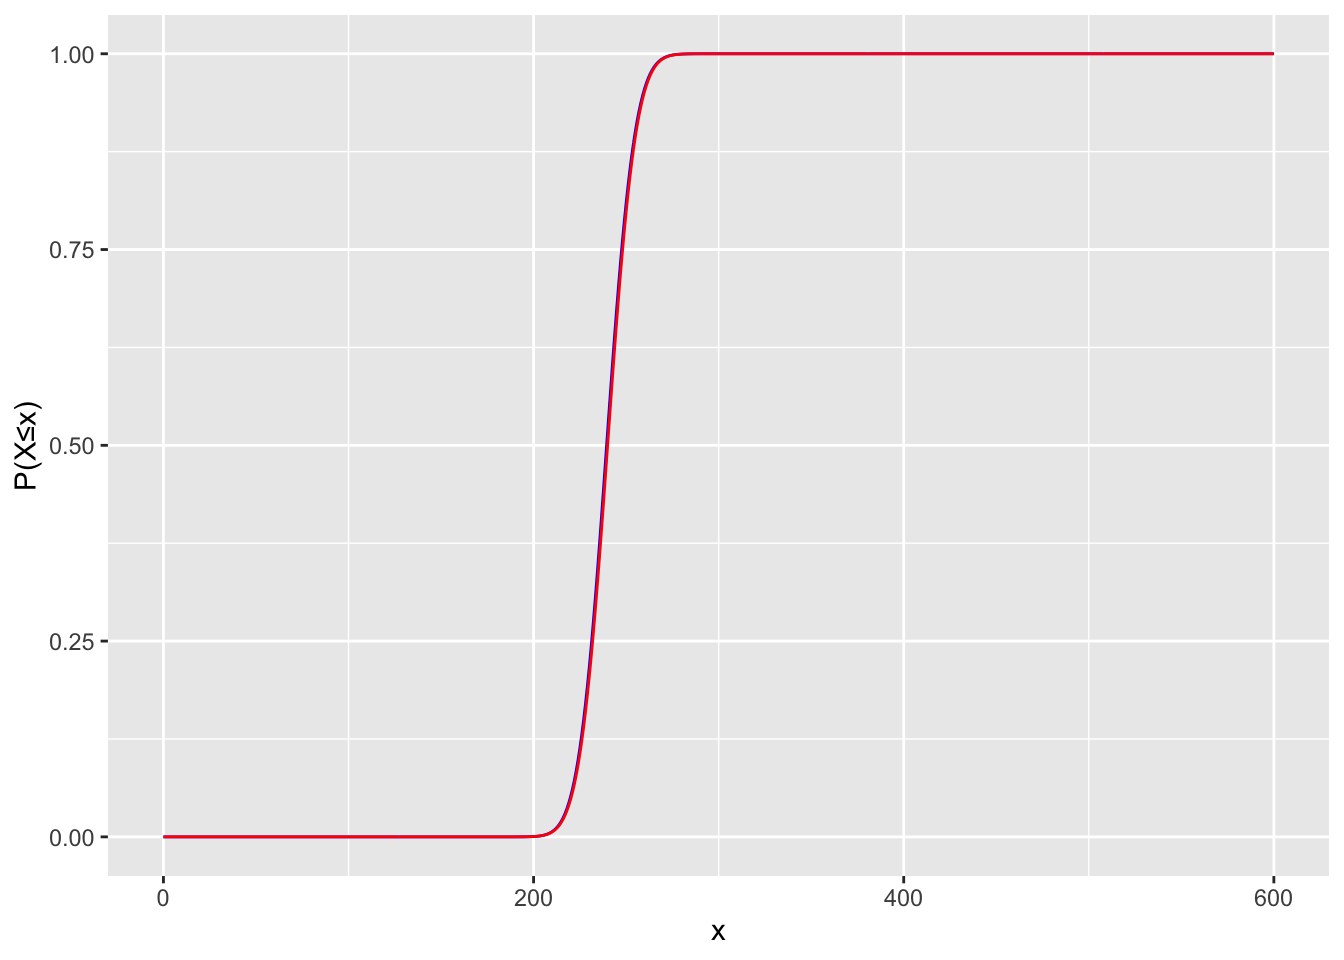
\includegraphics{_main_files/figure-latex/normal_binom_approx-1.pdf}

Visually, the CDFs appear to be very close to each other. You can compute their maximum difference to get a better idea how much they differ:

\begin{Shaded}
\begin{Highlighting}[]
\CommentTok{\#what\textquotesingle{}s the biggest difference between the two CDFs?}
\FunctionTok{max}\NormalTok{(}\FunctionTok{abs}\NormalTok{(bin\_cdf}\SpecialCharTok{{-}}\NormalTok{norm\_cdf))}
\end{Highlighting}
\end{Shaded}

\begin{verbatim}
## [1] 0.01772144
\end{verbatim}

\begin{Shaded}
\begin{Highlighting}[]
\CommentTok{\#for what value of x do they differ the most?}
\NormalTok{x\_vals[}\FunctionTok{which}\NormalTok{(}\FunctionTok{abs}\NormalTok{(bin\_cdf}\SpecialCharTok{{-}}\NormalTok{norm\_cdf)}\SpecialCharTok{==}\FunctionTok{max}\NormalTok{(}\FunctionTok{abs}\NormalTok{(bin\_cdf}\SpecialCharTok{{-}}\NormalTok{norm\_cdf)))]}
\end{Highlighting}
\end{Shaded}

\begin{verbatim}
## [1] 240
\end{verbatim}

Hence, the two CDFs are furthest apart for \(x=240\), with an absolute difference of 0.0177.

Now, try to approximate the variable \(X \sim \mbox{Bin}(n=30,\theta=0.2)\) with the distribution \(Y \sim N\left(\mu=n \times \theta,\sigma=\sqrt{n \times \theta \times (1-\theta)}\right)\). Compute the CDFs as in the code chunk above, and place the two CDFs on the same plot to answer the question that is to follow.

Hint

\begin{Shaded}
\begin{Highlighting}[]
\NormalTok{x\_vals }\OtherTok{\textless{}{-}} \FunctionTok{seq}\NormalTok{(}\AttributeTok{from=}\DecValTok{0}\NormalTok{,}\AttributeTok{to=}\DecValTok{30}\NormalTok{,}\AttributeTok{by=}\DecValTok{1}\NormalTok{)}
\NormalTok{bin\_cdf }\OtherTok{\textless{}{-}} \FunctionTok{pbinom}\NormalTok{(}\AttributeTok{q=}\NormalTok{x\_vals,}\AttributeTok{size=}\DecValTok{30}\NormalTok{,}\AttributeTok{prob=}\FloatTok{0.2}\NormalTok{)}
\NormalTok{norm\_cdf }\OtherTok{\textless{}{-}} \FunctionTok{pnorm}\NormalTok{(}\AttributeTok{q=}\NormalTok{x\_vals,}\AttributeTok{mean=}\DecValTok{6}\NormalTok{,}\AttributeTok{sd=}\FloatTok{2.19089}\NormalTok{)}

\NormalTok{cdfs }\OtherTok{\textless{}{-}} \FunctionTok{as.data.frame}\NormalTok{(}\FunctionTok{cbind}\NormalTok{(x\_vals,bin\_cdf,norm\_cdf))}

\CommentTok{\#Now use these to make the appropriate plot.}
\end{Highlighting}
\end{Shaded}

Solution

\begin{Shaded}
\begin{Highlighting}[]
\FunctionTok{ggplot}\NormalTok{(}\AttributeTok{data=}\NormalTok{cdfs) }\SpecialCharTok{+} \FunctionTok{geom\_line}\NormalTok{(}\FunctionTok{aes}\NormalTok{(x\_vals,bin\_cdf),}\AttributeTok{colour=}\StringTok{"blue"}\NormalTok{) }\SpecialCharTok{+} \FunctionTok{geom\_line}\NormalTok{(}\FunctionTok{aes}\NormalTok{(x\_vals,norm\_cdf),}\AttributeTok{colour=}\StringTok{"red"}\NormalTok{) }\SpecialCharTok{+} \FunctionTok{xlab}\NormalTok{(}\StringTok{"x"}\NormalTok{) }\SpecialCharTok{+} \FunctionTok{ylab}\NormalTok{(}\StringTok{"P(X≤x)"}\NormalTok{) }
\end{Highlighting}
\end{Shaded}

\begin{verbatim}
## Warning in grid.Call(C_textBounds, as.graphicsAnnot(x$label), x$x, x$y, :
## conversion failure on 'P(X≤x)' in 'mbcsToSbcs': dot substituted for <e2>
\end{verbatim}

\begin{verbatim}
## Warning in grid.Call(C_textBounds, as.graphicsAnnot(x$label), x$x, x$y, :
## conversion failure on 'P(X≤x)' in 'mbcsToSbcs': dot substituted for <89>
\end{verbatim}

\begin{verbatim}
## Warning in grid.Call(C_textBounds, as.graphicsAnnot(x$label), x$x, x$y, :
## conversion failure on 'P(X≤x)' in 'mbcsToSbcs': dot substituted for <a4>
\end{verbatim}

\begin{verbatim}
## Warning in grid.Call(C_textBounds, as.graphicsAnnot(x$label), x$x, x$y, :
## conversion failure on 'P(X≤x)' in 'mbcsToSbcs': dot substituted for <e2>
\end{verbatim}

\begin{verbatim}
## Warning in grid.Call(C_textBounds, as.graphicsAnnot(x$label), x$x, x$y, :
## conversion failure on 'P(X≤x)' in 'mbcsToSbcs': dot substituted for <89>
\end{verbatim}

\begin{verbatim}
## Warning in grid.Call(C_textBounds, as.graphicsAnnot(x$label), x$x, x$y, :
## conversion failure on 'P(X≤x)' in 'mbcsToSbcs': dot substituted for <a4>
\end{verbatim}

\begin{verbatim}
## Warning in grid.Call(C_textBounds, as.graphicsAnnot(x$label), x$x, x$y, :
## conversion failure on 'P(X≤x)' in 'mbcsToSbcs': dot substituted for <e2>
\end{verbatim}

\begin{verbatim}
## Warning in grid.Call(C_textBounds, as.graphicsAnnot(x$label), x$x, x$y, :
## conversion failure on 'P(X≤x)' in 'mbcsToSbcs': dot substituted for <89>
\end{verbatim}

\begin{verbatim}
## Warning in grid.Call(C_textBounds, as.graphicsAnnot(x$label), x$x, x$y, :
## conversion failure on 'P(X≤x)' in 'mbcsToSbcs': dot substituted for <a4>
\end{verbatim}

\begin{verbatim}
## Warning in grid.Call(C_textBounds, as.graphicsAnnot(x$label), x$x, x$y, :
## conversion failure on 'P(X≤x)' in 'mbcsToSbcs': dot substituted for <e2>
\end{verbatim}

\begin{verbatim}
## Warning in grid.Call(C_textBounds, as.graphicsAnnot(x$label), x$x, x$y, :
## conversion failure on 'P(X≤x)' in 'mbcsToSbcs': dot substituted for <89>
\end{verbatim}

\begin{verbatim}
## Warning in grid.Call(C_textBounds, as.graphicsAnnot(x$label), x$x, x$y, :
## conversion failure on 'P(X≤x)' in 'mbcsToSbcs': dot substituted for <a4>
\end{verbatim}

\begin{verbatim}
## Warning in grid.Call(C_textBounds, as.graphicsAnnot(x$label), x$x, x$y, :
## conversion failure on 'P(X≤x)' in 'mbcsToSbcs': dot substituted for <e2>
\end{verbatim}

\begin{verbatim}
## Warning in grid.Call(C_textBounds, as.graphicsAnnot(x$label), x$x, x$y, :
## conversion failure on 'P(X≤x)' in 'mbcsToSbcs': dot substituted for <89>
\end{verbatim}

\begin{verbatim}
## Warning in grid.Call(C_textBounds, as.graphicsAnnot(x$label), x$x, x$y, :
## conversion failure on 'P(X≤x)' in 'mbcsToSbcs': dot substituted for <a4>
\end{verbatim}

\begin{verbatim}
## Warning in grid.Call(C_textBounds, as.graphicsAnnot(x$label), x$x, x$y, :
## conversion failure on 'P(X≤x)' in 'mbcsToSbcs': dot substituted for <e2>
\end{verbatim}

\begin{verbatim}
## Warning in grid.Call(C_textBounds, as.graphicsAnnot(x$label), x$x, x$y, :
## conversion failure on 'P(X≤x)' in 'mbcsToSbcs': dot substituted for <89>
\end{verbatim}

\begin{verbatim}
## Warning in grid.Call(C_textBounds, as.graphicsAnnot(x$label), x$x, x$y, :
## conversion failure on 'P(X≤x)' in 'mbcsToSbcs': dot substituted for <a4>
\end{verbatim}

\begin{verbatim}
## Warning in grid.Call(C_textBounds, as.graphicsAnnot(x$label), x$x, x$y, :
## conversion failure on 'P(X≤x)' in 'mbcsToSbcs': dot substituted for <e2>
\end{verbatim}

\begin{verbatim}
## Warning in grid.Call(C_textBounds, as.graphicsAnnot(x$label), x$x, x$y, :
## conversion failure on 'P(X≤x)' in 'mbcsToSbcs': dot substituted for <89>
\end{verbatim}

\begin{verbatim}
## Warning in grid.Call(C_textBounds, as.graphicsAnnot(x$label), x$x, x$y, :
## conversion failure on 'P(X≤x)' in 'mbcsToSbcs': dot substituted for <a4>
\end{verbatim}

\begin{verbatim}
## Warning in grid.Call.graphics(C_text, as.graphicsAnnot(x$label), x$x, x$y, :
## conversion failure on 'P(X≤x)' in 'mbcsToSbcs': dot substituted for <e2>
\end{verbatim}

\begin{verbatim}
## Warning in grid.Call.graphics(C_text, as.graphicsAnnot(x$label), x$x, x$y, :
## conversion failure on 'P(X≤x)' in 'mbcsToSbcs': dot substituted for <89>
\end{verbatim}

\begin{verbatim}
## Warning in grid.Call.graphics(C_text, as.graphicsAnnot(x$label), x$x, x$y, :
## conversion failure on 'P(X≤x)' in 'mbcsToSbcs': dot substituted for <a4>
\end{verbatim}

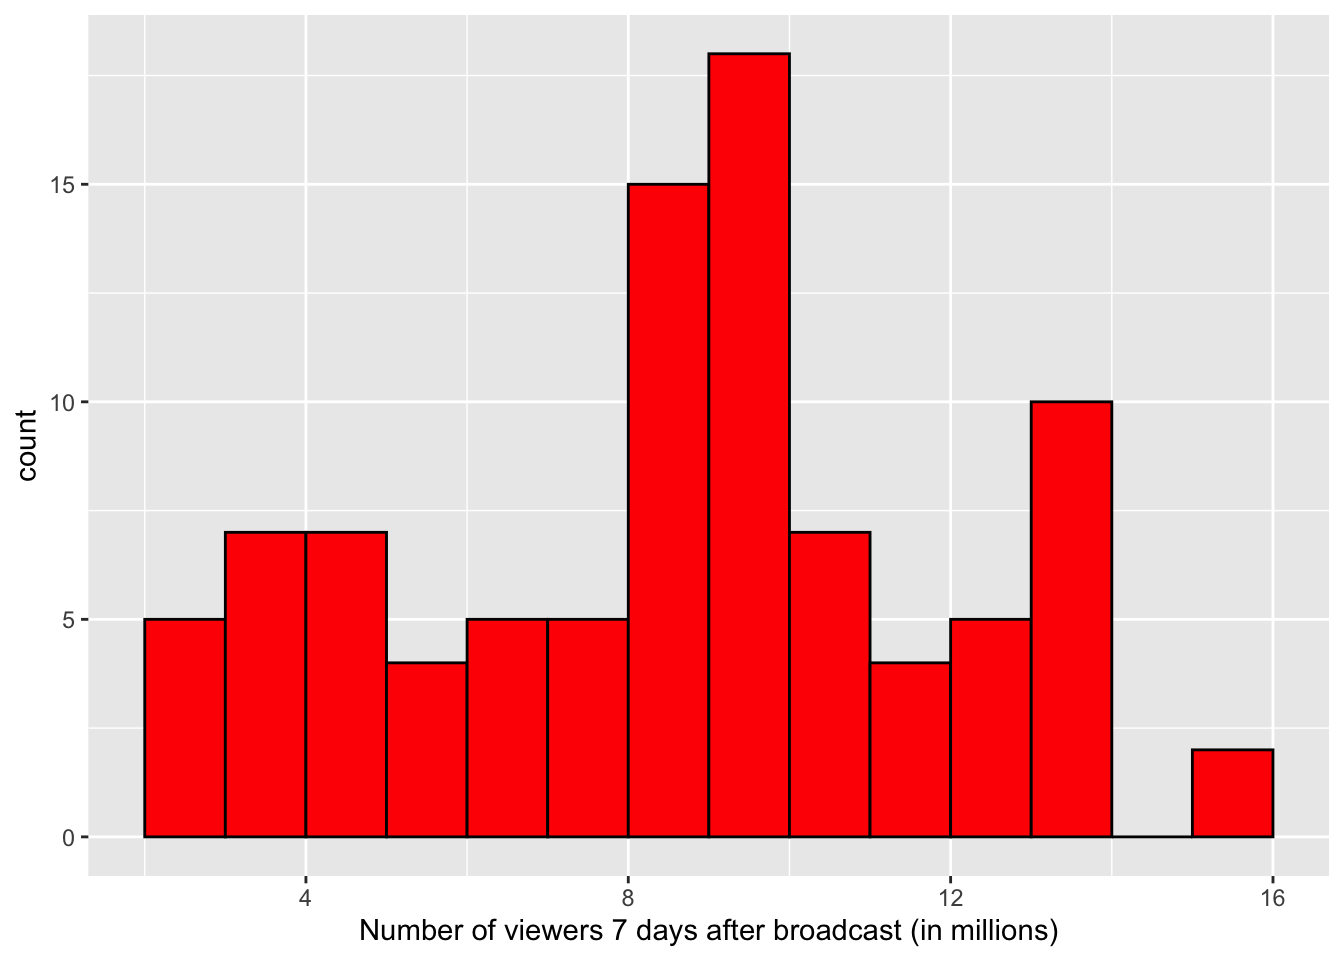
\includegraphics{_main_files/figure-latex/unnamed-chunk-14-1.pdf}

\textbf{Which of the following best describes the normal approximation for the binomial example under consideration?}

Hint

Is one of the coloured lines consistently higher than the other? If so, which one?

\begin{itemize}
\item
  \begin{enumerate}
  \def\labelenumi{(\Alph{enumi})}
  \tightlist
  \item
    The binomial CDF returns higher probabilities than the normal CDF for most values of x.\\
  \end{enumerate}
\item
  \begin{enumerate}
  \def\labelenumi{(\Alph{enumi})}
  \setcounter{enumi}{1}
  \tightlist
  \item
    The binomial CDF returns lower probabilities than the normal CDF for most values of x.\\
  \end{enumerate}
\item
  \begin{enumerate}
  \def\labelenumi{(\Alph{enumi})}
  \setcounter{enumi}{2}
  \tightlist
  \item
    While the approximation is not very accurate, sometimes the binomial CDF returns higher probabilities than the normal CDF, and sometimes it is the other way around.
  \end{enumerate}
\end{itemize}

Let's see how the probability of success \(\theta\) influences the dynamic of the normal approximation. Try to approximate the variable \(X \sim \mbox{Bin}(n=30,\theta=0.8)\) by \(Y \sim N\left(\mu=n \times \theta,\sigma=\sqrt{n \times \theta \times (1-\theta)}\right)\) and answer the question that is to follow.

Hint

\begin{Shaded}
\begin{Highlighting}[]
\NormalTok{x\_vals }\OtherTok{\textless{}{-}} \FunctionTok{seq}\NormalTok{(}\AttributeTok{from=}\DecValTok{0}\NormalTok{,}\AttributeTok{to=}\DecValTok{30}\NormalTok{,}\AttributeTok{by=}\DecValTok{1}\NormalTok{)}
\NormalTok{bin\_cdf }\OtherTok{\textless{}{-}} \FunctionTok{pbinom}\NormalTok{(}\AttributeTok{q=}\NormalTok{x\_vals,}\AttributeTok{size=}\DecValTok{30}\NormalTok{,}\AttributeTok{prob=}\FloatTok{0.8}\NormalTok{)}
\NormalTok{norm\_cdf }\OtherTok{\textless{}{-}} \FunctionTok{pnorm}\NormalTok{(}\AttributeTok{q=}\NormalTok{x\_vals,}\AttributeTok{mean=}\DecValTok{24}\NormalTok{,}\AttributeTok{sd=}\FloatTok{2.19089}\NormalTok{)}

\NormalTok{cdfs }\OtherTok{\textless{}{-}} \FunctionTok{as.data.frame}\NormalTok{(}\FunctionTok{cbind}\NormalTok{(x\_vals,bin\_cdf,norm\_cdf))}

\CommentTok{\#Now use these to make the appropriate plot.}
\end{Highlighting}
\end{Shaded}

Solution

\begin{Shaded}
\begin{Highlighting}[]
\FunctionTok{ggplot}\NormalTok{(}\AttributeTok{data=}\NormalTok{cdfs) }\SpecialCharTok{+} \FunctionTok{geom\_line}\NormalTok{(}\FunctionTok{aes}\NormalTok{(x\_vals,bin\_cdf),}\AttributeTok{colour=}\StringTok{"blue"}\NormalTok{) }\SpecialCharTok{+} \FunctionTok{geom\_line}\NormalTok{(}\FunctionTok{aes}\NormalTok{(x\_vals,norm\_cdf),}\AttributeTok{colour=}\StringTok{"red"}\NormalTok{) }\SpecialCharTok{+} \FunctionTok{xlab}\NormalTok{(}\StringTok{"x"}\NormalTok{) }\SpecialCharTok{+} \FunctionTok{ylab}\NormalTok{(}\StringTok{"P(X≤x)"}\NormalTok{) }
\end{Highlighting}
\end{Shaded}

\begin{verbatim}
## Warning in grid.Call(C_textBounds, as.graphicsAnnot(x$label), x$x, x$y, :
## conversion failure on 'P(X≤x)' in 'mbcsToSbcs': dot substituted for <e2>
\end{verbatim}

\begin{verbatim}
## Warning in grid.Call(C_textBounds, as.graphicsAnnot(x$label), x$x, x$y, :
## conversion failure on 'P(X≤x)' in 'mbcsToSbcs': dot substituted for <89>
\end{verbatim}

\begin{verbatim}
## Warning in grid.Call(C_textBounds, as.graphicsAnnot(x$label), x$x, x$y, :
## conversion failure on 'P(X≤x)' in 'mbcsToSbcs': dot substituted for <a4>
\end{verbatim}

\begin{verbatim}
## Warning in grid.Call(C_textBounds, as.graphicsAnnot(x$label), x$x, x$y, :
## conversion failure on 'P(X≤x)' in 'mbcsToSbcs': dot substituted for <e2>
\end{verbatim}

\begin{verbatim}
## Warning in grid.Call(C_textBounds, as.graphicsAnnot(x$label), x$x, x$y, :
## conversion failure on 'P(X≤x)' in 'mbcsToSbcs': dot substituted for <89>
\end{verbatim}

\begin{verbatim}
## Warning in grid.Call(C_textBounds, as.graphicsAnnot(x$label), x$x, x$y, :
## conversion failure on 'P(X≤x)' in 'mbcsToSbcs': dot substituted for <a4>
\end{verbatim}

\begin{verbatim}
## Warning in grid.Call(C_textBounds, as.graphicsAnnot(x$label), x$x, x$y, :
## conversion failure on 'P(X≤x)' in 'mbcsToSbcs': dot substituted for <e2>
\end{verbatim}

\begin{verbatim}
## Warning in grid.Call(C_textBounds, as.graphicsAnnot(x$label), x$x, x$y, :
## conversion failure on 'P(X≤x)' in 'mbcsToSbcs': dot substituted for <89>
\end{verbatim}

\begin{verbatim}
## Warning in grid.Call(C_textBounds, as.graphicsAnnot(x$label), x$x, x$y, :
## conversion failure on 'P(X≤x)' in 'mbcsToSbcs': dot substituted for <a4>
\end{verbatim}

\begin{verbatim}
## Warning in grid.Call(C_textBounds, as.graphicsAnnot(x$label), x$x, x$y, :
## conversion failure on 'P(X≤x)' in 'mbcsToSbcs': dot substituted for <e2>
\end{verbatim}

\begin{verbatim}
## Warning in grid.Call(C_textBounds, as.graphicsAnnot(x$label), x$x, x$y, :
## conversion failure on 'P(X≤x)' in 'mbcsToSbcs': dot substituted for <89>
\end{verbatim}

\begin{verbatim}
## Warning in grid.Call(C_textBounds, as.graphicsAnnot(x$label), x$x, x$y, :
## conversion failure on 'P(X≤x)' in 'mbcsToSbcs': dot substituted for <a4>
\end{verbatim}

\begin{verbatim}
## Warning in grid.Call(C_textBounds, as.graphicsAnnot(x$label), x$x, x$y, :
## conversion failure on 'P(X≤x)' in 'mbcsToSbcs': dot substituted for <e2>
\end{verbatim}

\begin{verbatim}
## Warning in grid.Call(C_textBounds, as.graphicsAnnot(x$label), x$x, x$y, :
## conversion failure on 'P(X≤x)' in 'mbcsToSbcs': dot substituted for <89>
\end{verbatim}

\begin{verbatim}
## Warning in grid.Call(C_textBounds, as.graphicsAnnot(x$label), x$x, x$y, :
## conversion failure on 'P(X≤x)' in 'mbcsToSbcs': dot substituted for <a4>
\end{verbatim}

\begin{verbatim}
## Warning in grid.Call(C_textBounds, as.graphicsAnnot(x$label), x$x, x$y, :
## conversion failure on 'P(X≤x)' in 'mbcsToSbcs': dot substituted for <e2>
\end{verbatim}

\begin{verbatim}
## Warning in grid.Call(C_textBounds, as.graphicsAnnot(x$label), x$x, x$y, :
## conversion failure on 'P(X≤x)' in 'mbcsToSbcs': dot substituted for <89>
\end{verbatim}

\begin{verbatim}
## Warning in grid.Call(C_textBounds, as.graphicsAnnot(x$label), x$x, x$y, :
## conversion failure on 'P(X≤x)' in 'mbcsToSbcs': dot substituted for <a4>
\end{verbatim}

\begin{verbatim}
## Warning in grid.Call(C_textBounds, as.graphicsAnnot(x$label), x$x, x$y, :
## conversion failure on 'P(X≤x)' in 'mbcsToSbcs': dot substituted for <e2>
\end{verbatim}

\begin{verbatim}
## Warning in grid.Call(C_textBounds, as.graphicsAnnot(x$label), x$x, x$y, :
## conversion failure on 'P(X≤x)' in 'mbcsToSbcs': dot substituted for <89>
\end{verbatim}

\begin{verbatim}
## Warning in grid.Call(C_textBounds, as.graphicsAnnot(x$label), x$x, x$y, :
## conversion failure on 'P(X≤x)' in 'mbcsToSbcs': dot substituted for <a4>
\end{verbatim}

\begin{verbatim}
## Warning in grid.Call.graphics(C_text, as.graphicsAnnot(x$label), x$x, x$y, :
## conversion failure on 'P(X≤x)' in 'mbcsToSbcs': dot substituted for <e2>
\end{verbatim}

\begin{verbatim}
## Warning in grid.Call.graphics(C_text, as.graphicsAnnot(x$label), x$x, x$y, :
## conversion failure on 'P(X≤x)' in 'mbcsToSbcs': dot substituted for <89>
\end{verbatim}

\begin{verbatim}
## Warning in grid.Call.graphics(C_text, as.graphicsAnnot(x$label), x$x, x$y, :
## conversion failure on 'P(X≤x)' in 'mbcsToSbcs': dot substituted for <a4>
\end{verbatim}

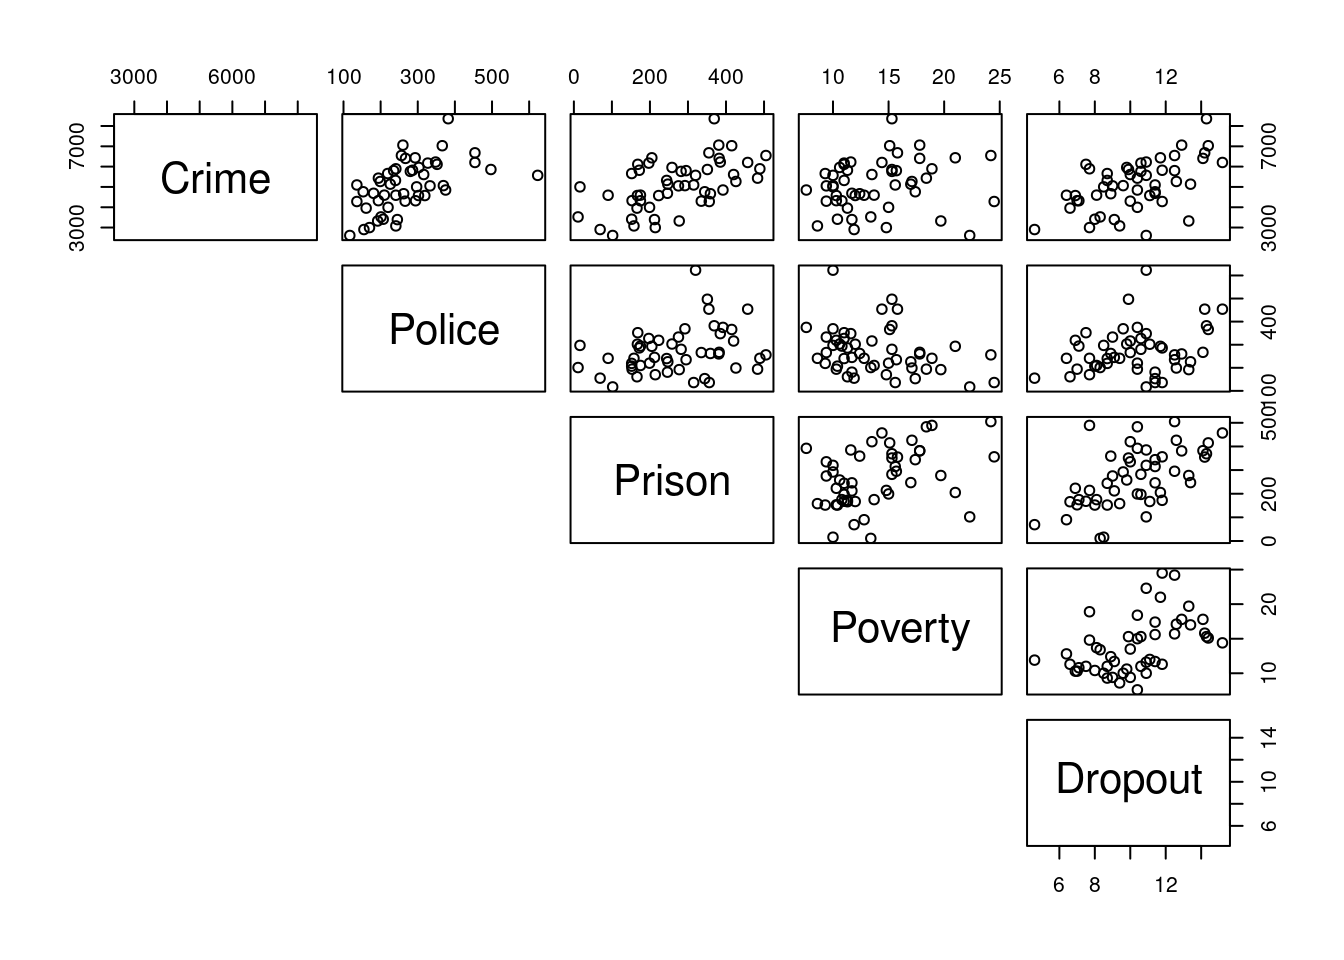
\includegraphics{_main_files/figure-latex/unnamed-chunk-17-1.pdf}

\textbf{Now that we have increased the probability of success to \(\theta=0.8\), which of the following best describes the Normal approximation for the Binomial example under consideration?}

Hint

Is one of the coloured lines consistently higher than the other? If so, which one?

\begin{itemize}
\item
  \begin{enumerate}
  \def\labelenumi{(\Alph{enumi})}
  \tightlist
  \item
    The binomial CDF still returns higher probabilities than the normal CDF for most values of x.\\
  \end{enumerate}
\item
  \begin{enumerate}
  \def\labelenumi{(\Alph{enumi})}
  \setcounter{enumi}{1}
  \tightlist
  \item
    The binomial CDF now returns lower probabilities than the normal CDF for most values of x.\\
  \end{enumerate}
\item
  \begin{enumerate}
  \def\labelenumi{(\Alph{enumi})}
  \setcounter{enumi}{2}
  \tightlist
  \item
    While the approximation is still not very accurate, now the binomial CDF sometimes returns higher probabilities than the normal CDF, and sometimes it is the other way around.
  \end{enumerate}
\end{itemize}

Sometimes, when computations become increasingly expensive, it can be quite useful to approximate the binomial distribution by a normal distribution. Hopefully, this part of the lab helped you understand why the normal approximation is only appropriate when the number of observations \(n\) is sufficiently large for a given probability of success \(\theta\). Keeping this in mind, you should always check the assumptions \(n \times \theta \geq 10\) and \(n \times (1-\theta) \geq 10\) before applying the normal approximation and compute the binomial probabilities directly if the assumptions do not hold.

\hypertarget{group-exercises}{%
\chapter{Group Exercises}\label{group-exercises}}

In this group exercise, you will generate random samples from normal distributions. You will then pretend the samples had been handed to you, and explore the samples visually to examine whether the normality assumption seems appropriate for the sample at hand. You might find this exercise helpful in the preparation for later parts of the course, where you will be given a sample or dataset and asked to check if the normality assumption is appropriate for some variable, before performing tests that assume an underlying normal distribution.

In \texttt{R}, you can generate random values from several probability distributions. For example, you can use the functions \texttt{rbinom()} and \texttt{rpois()} to obtain random values from the binomial and Poisson distributions, respectively. Similarly, you can obtain random values from a normal distribution using the function \texttt{rnorm()}.

Note: the function \texttt{rnorm()} returns random values from the specified probability distribution, so your results of the following simulation study will vary every time you run the code. The questions for this exercise are based on a seed of 1 (setting a seed allows for reproducibility of results obtained from random functions), which is done via the command \texttt{set.seed(1)}, which you should run before each random function in this exercise to ensure you can get to the correct answers.

For example, in the code below you will see that the results differ if you do not set a seed but that repeated trials lead to the same result if you use the same seed:

\begin{Shaded}
\begin{Highlighting}[]
\FunctionTok{set.seed}\NormalTok{(}\DecValTok{1}\NormalTok{)}
\FunctionTok{rnorm}\NormalTok{(}\AttributeTok{n=}\DecValTok{5}\NormalTok{,}\AttributeTok{mean=}\DecValTok{3}\NormalTok{,}\AttributeTok{sd=}\DecValTok{1}\NormalTok{)}
\end{Highlighting}
\end{Shaded}

\begin{verbatim}
## [1] 2.373546 3.183643 2.164371 4.595281 3.329508
\end{verbatim}

\begin{Shaded}
\begin{Highlighting}[]
\CommentTok{\#here, no seed was specified, so the result is different:}
\FunctionTok{rnorm}\NormalTok{(}\AttributeTok{n=}\DecValTok{5}\NormalTok{,}\AttributeTok{mean=}\DecValTok{3}\NormalTok{,}\AttributeTok{sd=}\DecValTok{1}\NormalTok{)}
\end{Highlighting}
\end{Shaded}

\begin{verbatim}
## [1] 2.179532 3.487429 3.738325 3.575781 2.694612
\end{verbatim}

\begin{Shaded}
\begin{Highlighting}[]
\CommentTok{\#using the same seed as before leads to the same result}
\FunctionTok{set.seed}\NormalTok{(}\DecValTok{1}\NormalTok{)}
\FunctionTok{rnorm}\NormalTok{(}\AttributeTok{n=}\DecValTok{5}\NormalTok{,}\AttributeTok{mean=}\DecValTok{3}\NormalTok{,}\AttributeTok{sd=}\DecValTok{1}\NormalTok{)}
\end{Highlighting}
\end{Shaded}

\begin{verbatim}
## [1] 2.373546 3.183643 2.164371 4.595281 3.329508
\end{verbatim}

\hypertarget{checking-the-normality-assumption}{%
\subsection{Checking the normality assumption}\label{checking-the-normality-assumption}}

\textbf{1. Generate 30 values from a normal distribution with mean \(\mu=10\) and variance \(\sigma^{2}=4\). Then, create a boxplot for your sample. Remember to set a seed of 1 before running the function.}

\textbf{2. Imagine you were handed the sample without being told that it was generated from a normal distribution. Based on the boxplot, would you say that the sample approximately follows a normal distribution?}

\begin{itemize}
\item
  \begin{enumerate}
  \def\labelenumi{(\Alph{enumi})}
  \tightlist
  \item
    The boxplot suggests it is unlikely that the majority of observations fall within one standard deviation of the mean. Hence, the normality assumption seems to be violated.\\
  \end{enumerate}
\item
  \begin{enumerate}
  \def\labelenumi{(\Alph{enumi})}
  \setcounter{enumi}{1}
  \tightlist
  \item
    The boxplot shows that the median is closer to the third quartile than to the first. However, the boxplot looks roughly symmetric and hence, the normality assumption seems appropriate.\\
  \end{enumerate}
\item
  \begin{enumerate}
  \def\labelenumi{(\Alph{enumi})}
  \setcounter{enumi}{2}
  \tightlist
  \item
    The minimum is further away from the median than the maximum. Hence, the sample does not seem to be symmetric and thus, it appears that the normality assumption is violated.
  \end{enumerate}
\end{itemize}

\textbf{3. Next, create a histogram to get a better idea of the shape of the distribution. You might have to change the binwidth to get a better plot.}

\textbf{4. Based on the histogram, would you say that the sample approximately follows a Normal distribution?}

\begin{itemize}
\item
  \begin{enumerate}
  \def\labelenumi{(\Alph{enumi})}
  \tightlist
  \item
    The lower tail of the distribution is slightly heavier than the upper tail. However, the data closer to the mode of the distribution seem roughly symmetric and hence, the normality assumption isn\textquotesingle t violated.\\
  \end{enumerate}
\item
  \begin{enumerate}
  \def\labelenumi{(\Alph{enumi})}
  \setcounter{enumi}{1}
  \tightlist
  \item
    It doesn\textquotesingle t look like the majority of data fall within one standard deviation of the mean. Hence, the normality assumption seems to be violated.\\
  \end{enumerate}
\item
  \begin{enumerate}
  \def\labelenumi{(\Alph{enumi})}
  \setcounter{enumi}{2}
  \tightlist
  \item
    The sample contains many very small values which make it unlikely that the data follow a Normal distribution.
  \end{enumerate}
\end{itemize}

\hypertarget{heights-in-the-scottish-population}{%
\subsection{Heights in the Scottish population}\label{heights-in-the-scottish-population}}

In Scotland, the average height for females is 161.3cm while that of males is 175cm. The standard deviation is approximately 6cm for females and 7cm for males.

\textbf{5. Based on this information, generate a random sample of the heights of 20 Scottish females and 20 Scottish males (remember to set a seed of 1 before you evaluate each function). Then, create a boxplot for the heights of the 40 people in the sample.}

\textbf{6. Imagine you were handed the sample without being told that it was generated from a Normal distribution. Based on the boxplot, would you say that the sample approximately follows a normal distribution?}

\begin{itemize}
\item
  \begin{enumerate}
  \def\labelenumi{(\Alph{enumi})}
  \tightlist
  \item
    It doesn\textquotesingle t look like the majority of data fall within one standard deviation of the mean. Hence, the normality assumption seems to be violated.\\
  \end{enumerate}
\item
  \begin{enumerate}
  \def\labelenumi{(\Alph{enumi})}
  \setcounter{enumi}{1}
  \tightlist
  \item
    The boxplot does not look symmetric, as the third quartile is further away from the median than the fist. Hence, the normality assumption seems violated.\\
  \end{enumerate}
\item
  \begin{enumerate}
  \def\labelenumi{(\Alph{enumi})}
  \setcounter{enumi}{2}
  \tightlist
  \item
    The boxplot looks roughly symmetric and hence, the normality assumption seems appropriate.
  \end{enumerate}
\end{itemize}

\textbf{7. As before, create a histogram to get a better idea of the shape of the distribution. You might have to change the binwidth to get a better plot.}

\textbf{8. Based on the histogram, would you say that the sample approximately follows a normal distribution?}

\begin{itemize}
\item
  \begin{enumerate}
  \def\labelenumi{(\Alph{enumi})}
  \tightlist
  \item
    The normal distriution is unimodal and symmetric. The sample is not symmetric around a single mode and hence, the normality assumption seems violated.\\
  \end{enumerate}
\item
  \begin{enumerate}
  \def\labelenumi{(\Alph{enumi})}
  \setcounter{enumi}{1}
  \tightlist
  \item
    There are too many observations far below the median. Hence, the distribution does not look symmetric and the normality assumption seems violated.\\
  \end{enumerate}
\item
  \begin{enumerate}
  \def\labelenumi{(\Alph{enumi})}
  \setcounter{enumi}{2}
  \tightlist
  \item
    The sample is roughly symmetric. Hence, the normality assumption seems appropriate.
  \end{enumerate}
\end{itemize}

Hopefully, this exercise gave you a first idea on how to check the appropriateness of assuming normality of a sample. Also, you saw that it might be helpful considering different plots when evaluating whether the normality assumption is appropriate.

\end{document}
